\documentclass[11pt, a4paper]{report}

\usepackage[utf8]{inputenc} % allow characters like "ü" etc.
\usepackage[a4paper, left=20mm, right=20mm, top=20mm, bottom=20mm]{geometry} %format of the page
\usepackage{fancyhdr} %usage of header and footer
\usepackage{graphicx} %including images

% definition of the header/ footer
\pagestyle{empty}
\pagestyle{fancy}
\rhead{Author: Simon\_2}
\chead{Written Report - 6.419x Module 3}
%\rhead{\today}

\parindent 0pt % set indention to zero points

\begin{document}


	\textbf{Problem 2}\\
(c). (2 points) \textsl{Observe the plot you made in Part (a) Question 1. The number of nodes increases sharply over the first few phases then levels out. Comment on what you think may be causing this effect. Based on your answer, should you adjust your conclusions in Part (b) Question 5? ($\sim$100 words, 200 word limit.)}\\

\textbf{Solution}:\\
The number of nodes and edges of the network is increasing quite fast in the first three phases (see figure \ref{fig:nodes_edges}). The seizure of 300 kg of marijuana (phase 4) might have the effect of decreasing edge numbers and stagnating node counts. The phases of seizures seem to bound the number of edges to around 50 and reduces the growth rate of node counts.\\

\begin{figure}[h]
	\centering
	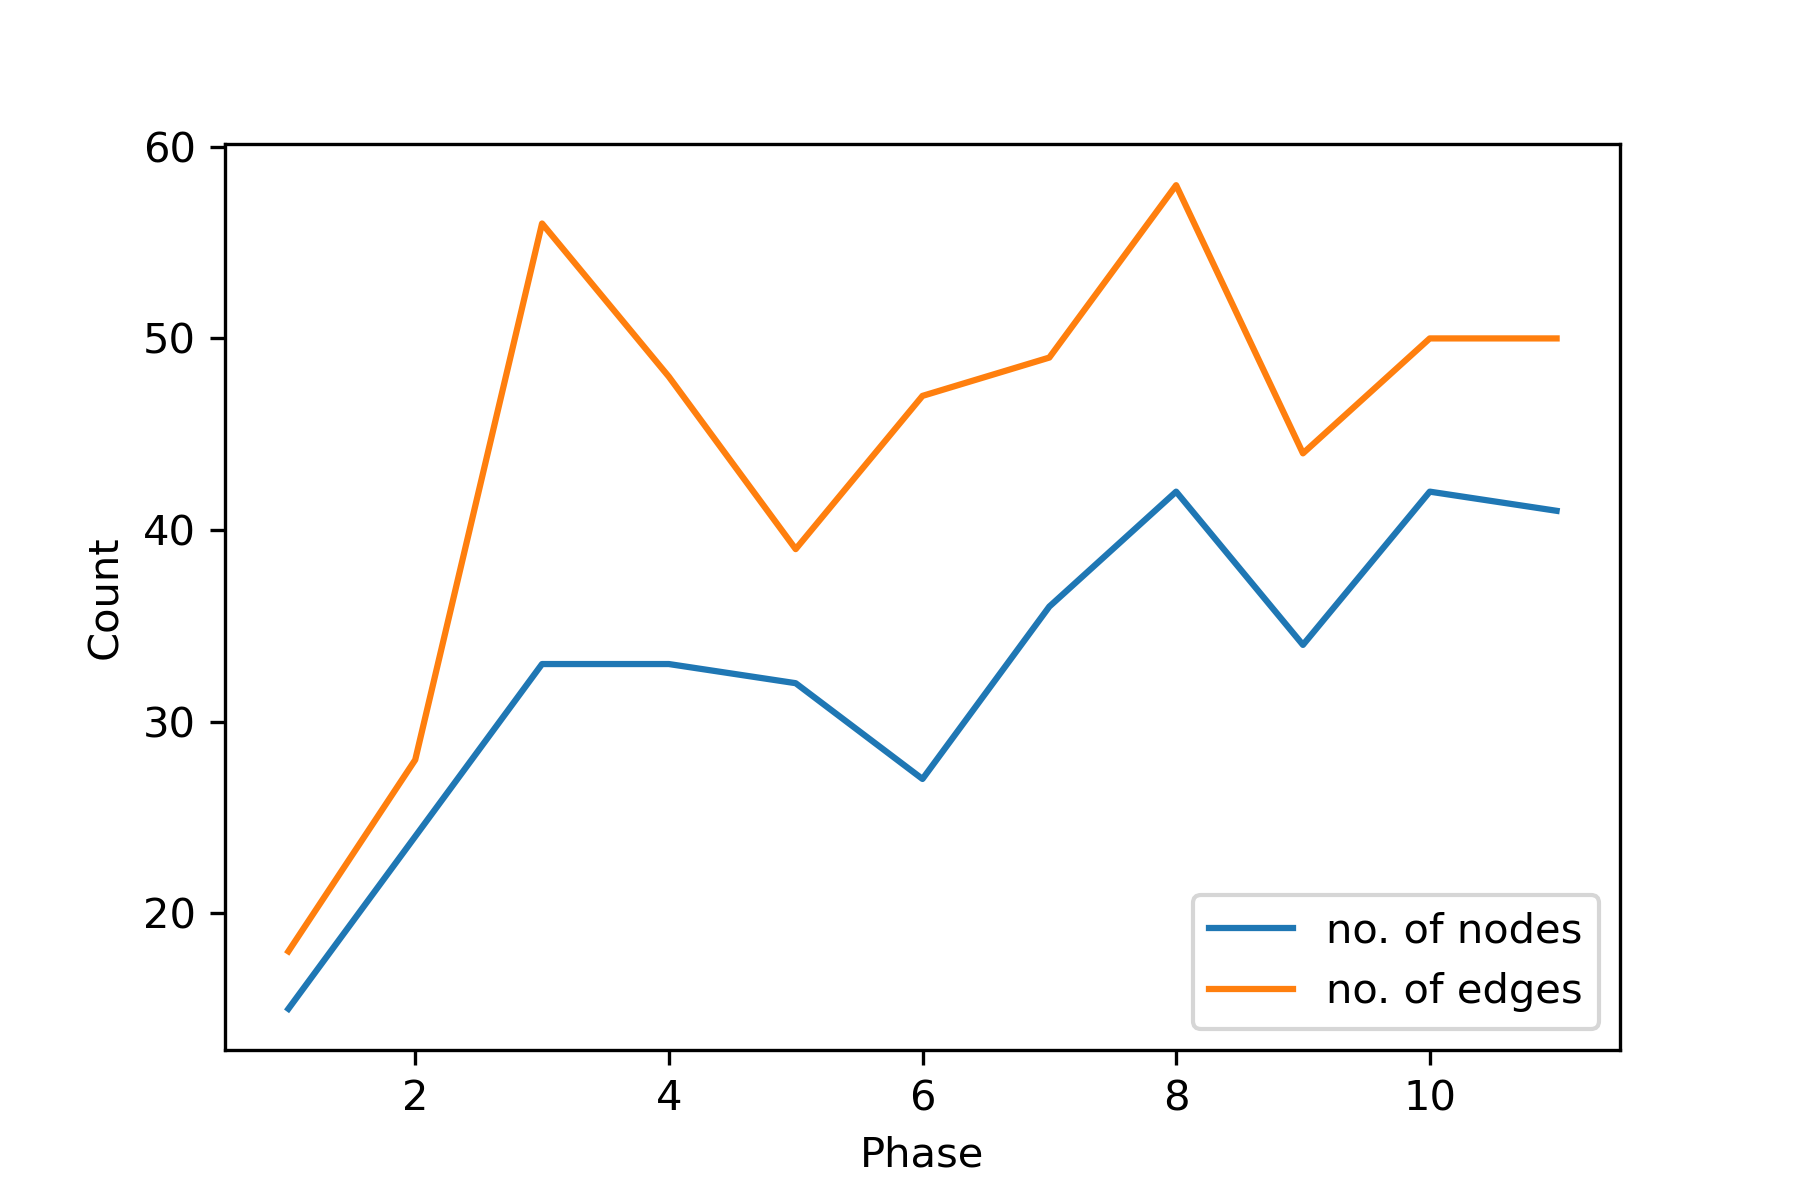
\includegraphics[width=0.7\linewidth]{problem_02/nodes_edges}
	\caption{Number of nodes and edges over phases}
	\label{fig:nodes_edges}
\end{figure}

The mean value of a centrality measure over all phases does not take into account how the individual node acts over phases. The importance of individual nodes could for example fade out over time, which is not represented by this model.\\
	\vspace{1cm}
	
	(d). (5 points) \textsl{In the context of criminal networks, what would each of these metrics teach you about the importance of an actor's role in the traffic? In your own words, could you explain the limitations of degree centrality? In your opinion, which one would be most relevant to identify who is running the illegal activities of the group? Please justify. ($\sim$300 words, 400 word limit.)}\\

\textbf{Solution}:\\
The degree centrality gives us information about the node which has the most edges to other nodes. But it does not differentiate between the importance of the connected nodes. This model would weigh two nodes with equal node numbers identically, even though one connects to "low-level" drug dealers (without further criminal connections) and one connects to "high-level" drug dealers (with multiple criminal connections).\\

This drawback can be bypassed by using the eigenvector centrality. This model takes into account to which nodes the representative node is connected to. In terms of a drug dealing network the individual node is more important if it is connected to multiple "high-level" rather than "low-level" drug dealers.\\

The betweenness centrality on the other hand tries to weigh how important one node is for the connection between other nodes. A node with a high betweenness centrality could be for example an individual node which connects multiple sub-graphs. If it is removed from the network, the whole network is weakened because it lost its "core" node.\\

When it comes to choose one individual as a so called "mastermind" who connects different groups of the network the betweenness centrality is an adequate indicator. As in the lecture described, a node with a high betweenness centrality breaks a network apart best when removed. And this is exactly what we try to achieve in terms of a criminal network.\\
	
	\newpage
	\textbf{Problem 2}\\
(c). (2 points) \textsl{Observe the plot you made in Part (a) Question 1. The number of nodes increases sharply over the first few phases then levels out. Comment on what you think may be causing this effect. Based on your answer, should you adjust your conclusions in Part (b) Question 5? ($\sim$100 words, 200 word limit.)}\\

\textbf{Solution}:\\
The number of nodes and edges of the network is increasing quite fast in the first three phases (see figure \ref{fig:nodes_edges}). The seizure of 300 kg of marijuana (phase 4) might have the effect of decreasing edge numbers and stagnating node counts. The phases of seizures seem to bound the number of edges to around 50 and reduces the growth rate of node counts.\\

\begin{figure}[h]
	\centering
	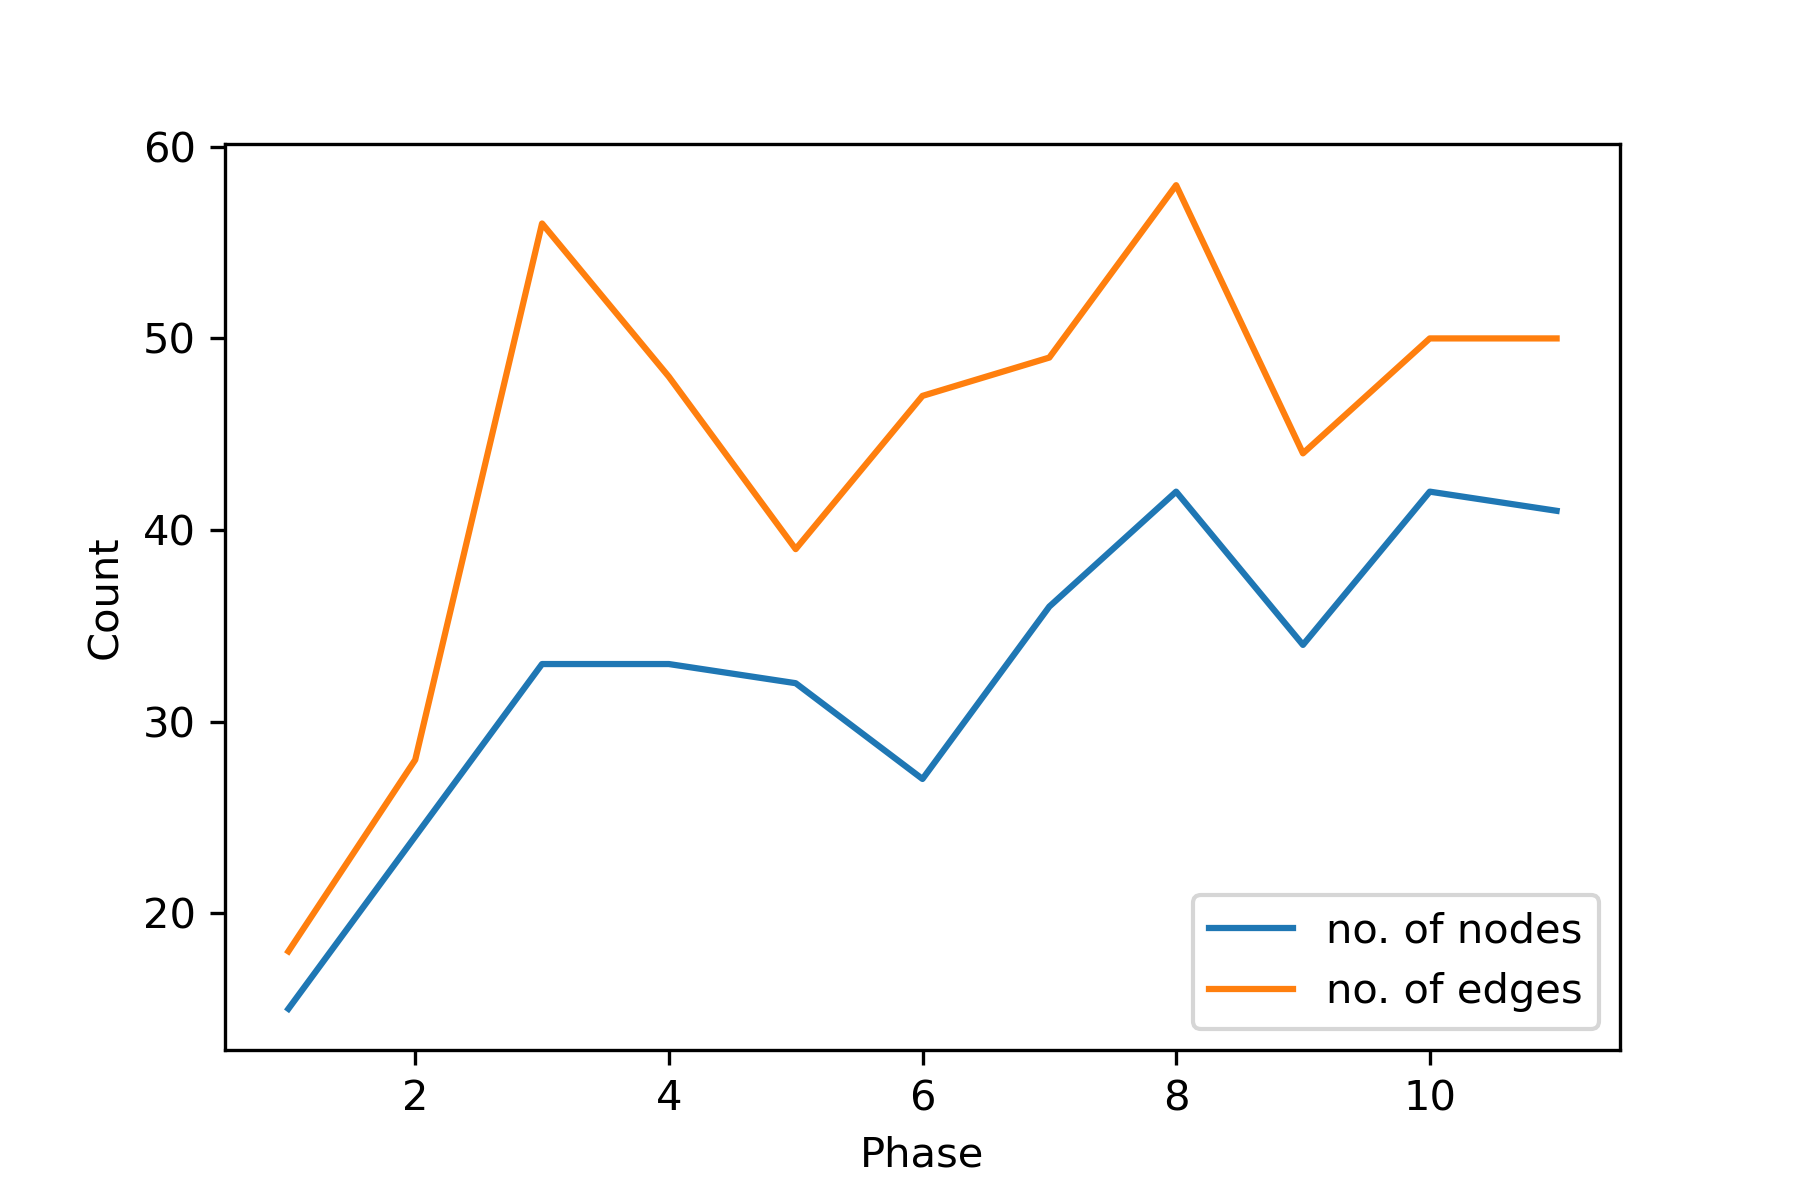
\includegraphics[width=0.7\linewidth]{problem_02/nodes_edges}
	\caption{Number of nodes and edges over phases}
	\label{fig:nodes_edges}
\end{figure}

The mean value of a centrality measure over all phases does not take into account how the individual node acts over phases. The importance of individual nodes could for example fade out over time, which is not represented by this model.\\
	\vspace{1cm}
		
	(d). (5 points) \textsl{In the context of criminal networks, what would each of these metrics teach you about the importance of an actor's role in the traffic? In your own words, could you explain the limitations of degree centrality? In your opinion, which one would be most relevant to identify who is running the illegal activities of the group? Please justify. ($\sim$300 words, 400 word limit.)}\\

\textbf{Solution}:\\
The degree centrality gives us information about the node which has the most edges to other nodes. But it does not differentiate between the importance of the connected nodes. This model would weigh two nodes with equal node numbers identically, even though one connects to "low-level" drug dealers (without further criminal connections) and one connects to "high-level" drug dealers (with multiple criminal connections).\\

This drawback can be bypassed by using the eigenvector centrality. This model takes into account to which nodes the representative node is connected to. In terms of a drug dealing network the individual node is more important if it is connected to multiple "high-level" rather than "low-level" drug dealers.\\

The betweenness centrality on the other hand tries to weigh how important one node is for the connection between other nodes. A node with a high betweenness centrality could be for example an individual node which connects multiple sub-graphs. If it is removed from the network, the whole network is weakened because it lost its "core" node.\\

When it comes to choose one individual as a so called "mastermind" who connects different groups of the network the betweenness centrality is an adequate indicator. As in the lecture described, a node with a high betweenness centrality breaks a network apart best when removed. And this is exactly what we try to achieve in terms of a criminal network.\\
	\vspace{1cm}	
	
	(e). (3 points) \textsl{In real life, the police need to effectively use all the information they have gathered, to identify who is responsible for running the illegal activities of the group. Armed with a qualitative understanding of the centrality metrics from Part (d) and the quantitative analysis from part Part (b) Question 5, integrate and interpret the information you have to identify which players were most central (or important) to the operation. ($\sim$100 words, 200 word limit.)}\\

\textbf{Solution}:\\
The comparison of different centrality mean values of all phases for all nodes represent the phase-average importance of individual nodes within the CAVIAR network (see table \ref{tab:centrality_important_nodes}). The importance of a node can be defined as the power to connect other nodes which increases each individuals influence.\\

\begin{table}[h]
	\centering
	\begin{tabular}{|c|c|c|c|}
		\hline 
		Centrality type & Highest & Second highest & Third highest \\ 
		\hline 
		Betweenness & no. 1 (0.66) & no. 12 (0.17) & no. 3 (0.13) \\ 
		\hline 
		Eigenvector & no. 1 (0.55) & no. 3 (0.30) & no. 85 (0.19)\\ 
		\hline 
	\end{tabular} 
	\caption{Comparison between different centrality measures and corresponding most important nodes (individuals of CAVIAR network, mean values over all phases)}
	\label{tab:centrality_important_nodes}
\end{table}

Both, mean betweenness and mean eigenvector centrality, state that node no. 1 is the most important node. As mentioned before, the betweenness centrality is a good indicator to judge on which individual the police should focus on. Therefore, the nodes no. 12 and 3 are the next two nodes, which should be persecuted.\\
	\vspace{1cm}
	
	(f). (3 points) \textsl{The change in the network from Phase X to X+1 coincides with a major event that took place during the actual investigation. Identify the event and explain how the change in centrality rankings and visual patterns, observed in the network plots above, relates to said event. ($\sim$200 words, 300 word limit.)}\\

\textbf{Solution}:\\
The network plot shows the change from phase 4 to 5. It shows the behavior of the CAVIAR network on the first seizure of 300 kg of marijuana with a value of 2,500,000\$. The five most important nodes show an interesting effect of the seizure on the network (see table \ref{tab:centrality_phase_4_5}). In both phases node number 1 is by far the most important node. But the second node changes. In phase 4 no. 89 is the second most important node. But in phase 5 it is not even listed under the top five. Number 89 is the investor Antonio Iannacci.\\

\begin{table}[!h]
	\centering
	\begin{tabular}{|c|c|c|}
		\hline 
		 & Phase 4 & Phase 5 \\ 
		\hline 
		1st most important node & no. 1 (0.84) & no. 1 (0.88)  \\ 
		\hline 
		2nd most important node & no. 89 (0.20) & no. 12 (0.30) \\ 
		\hline 
		3rd most important node & no. 3 (0.09) & no. 83 (0.06) \\ 
		\hline 
		4th most important node & no. 83 (0.08) & no. 31 (0.06) \\ 
		\hline 
		5th most important node & no. 13 (0.06) & no. 85 (0.06) \\ 
		\hline 
	\end{tabular} 
	\caption{Change of centrality measures from phase 4 to 5 (node number and corresponding betweenness centrality)}
	\label{tab:centrality_phase_4_5}
\end{table}

In contrast node number 12 jumps on the second place in phase 5, even though it was not listed in the top five in phase 4. The seizure of marijuana seems to have a beneficial effect on the criminal career of Ernesto Morales, the principal organizer of the cocaine import and intermediary between the Colombians and the Serero organization. After this event cocaine is regularly seized in several phases.\\

The visualization of the networks shows graphically that besides node no. 1, node no. 12 emerges in the network. Node no. 89 is still represented, but is not as essential as before. There are several alternative connections for this node, in contrast to phase 4.\\
	\vspace{1cm}
	
	(g). (4 points) \textsl{While centrality helps explain the evolution of every player's role individually, we need to explore the global trends and incidents in the story in order to understand the behavior of the criminal enterprise.}\\
\textsl{Describe the coarse pattern(s) you observe as the network evolves through the phases. Does the network evolution reflect the background story? ($\sim$200 words, 300 word limit.)}\\

\textbf{Solution}:\\
As mentioned before in part (c), the number of edges is not further increasing after phase 4, whereas the number of nodes is slowly increasing until it reaches a plateau-like boundary at phase 8 (see figure \ref{fig:nodes_edges}). This development can visually be shown in figure \ref{fig:network_visualization}. Generally there is a development that the network decentralizes over the phases and its main actor (node no. 1) looses his importance according to the betweenness centrality (see figure \ref{fig:betweenness_specific_nodes}). The seizures seem to have some impact on the structure of the graph.\\

\begin{figure}[htbp]
	\centering
	\begin{minipage}{.24\textwidth}
		\centering
		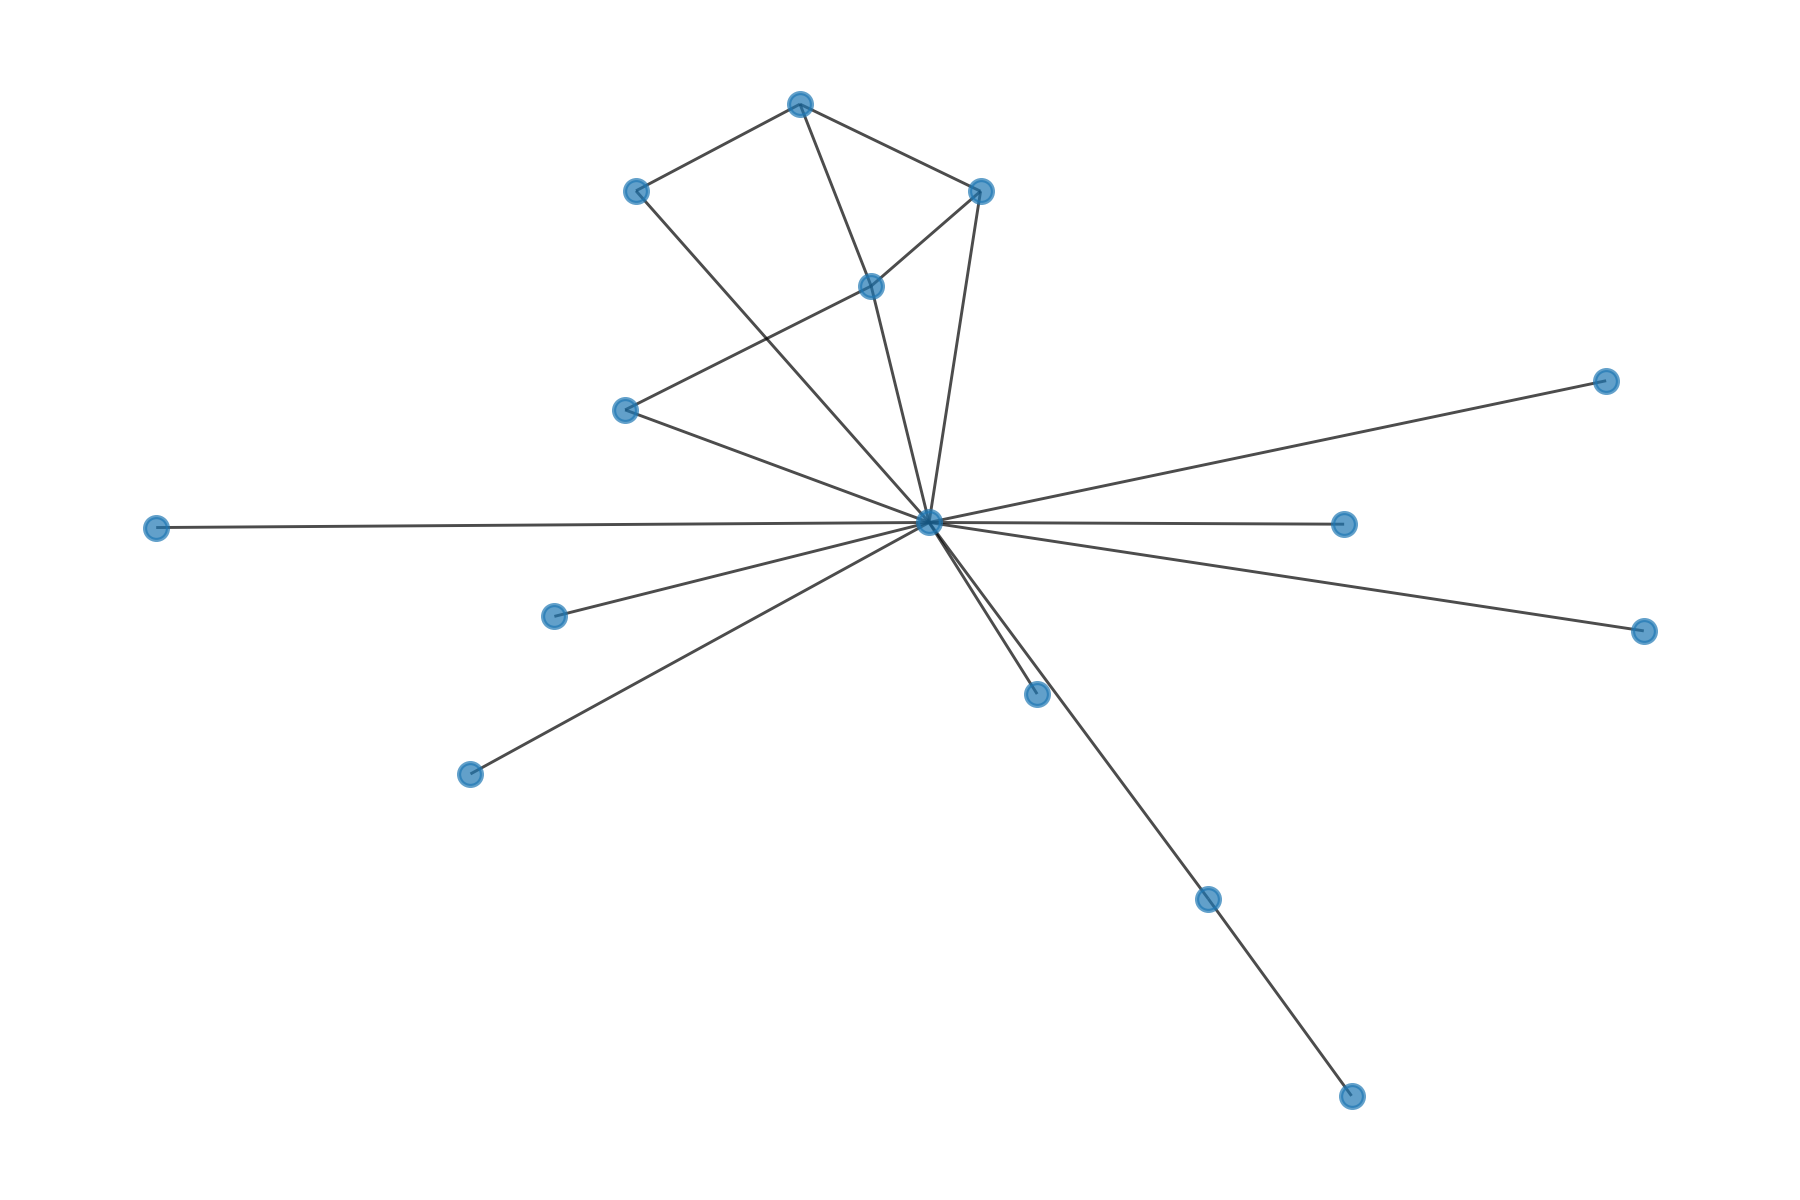
\includegraphics[width=1\linewidth]{problem_02/network_phase1}
	\end{minipage}
	\begin{minipage}{.24\textwidth}
		\centering
		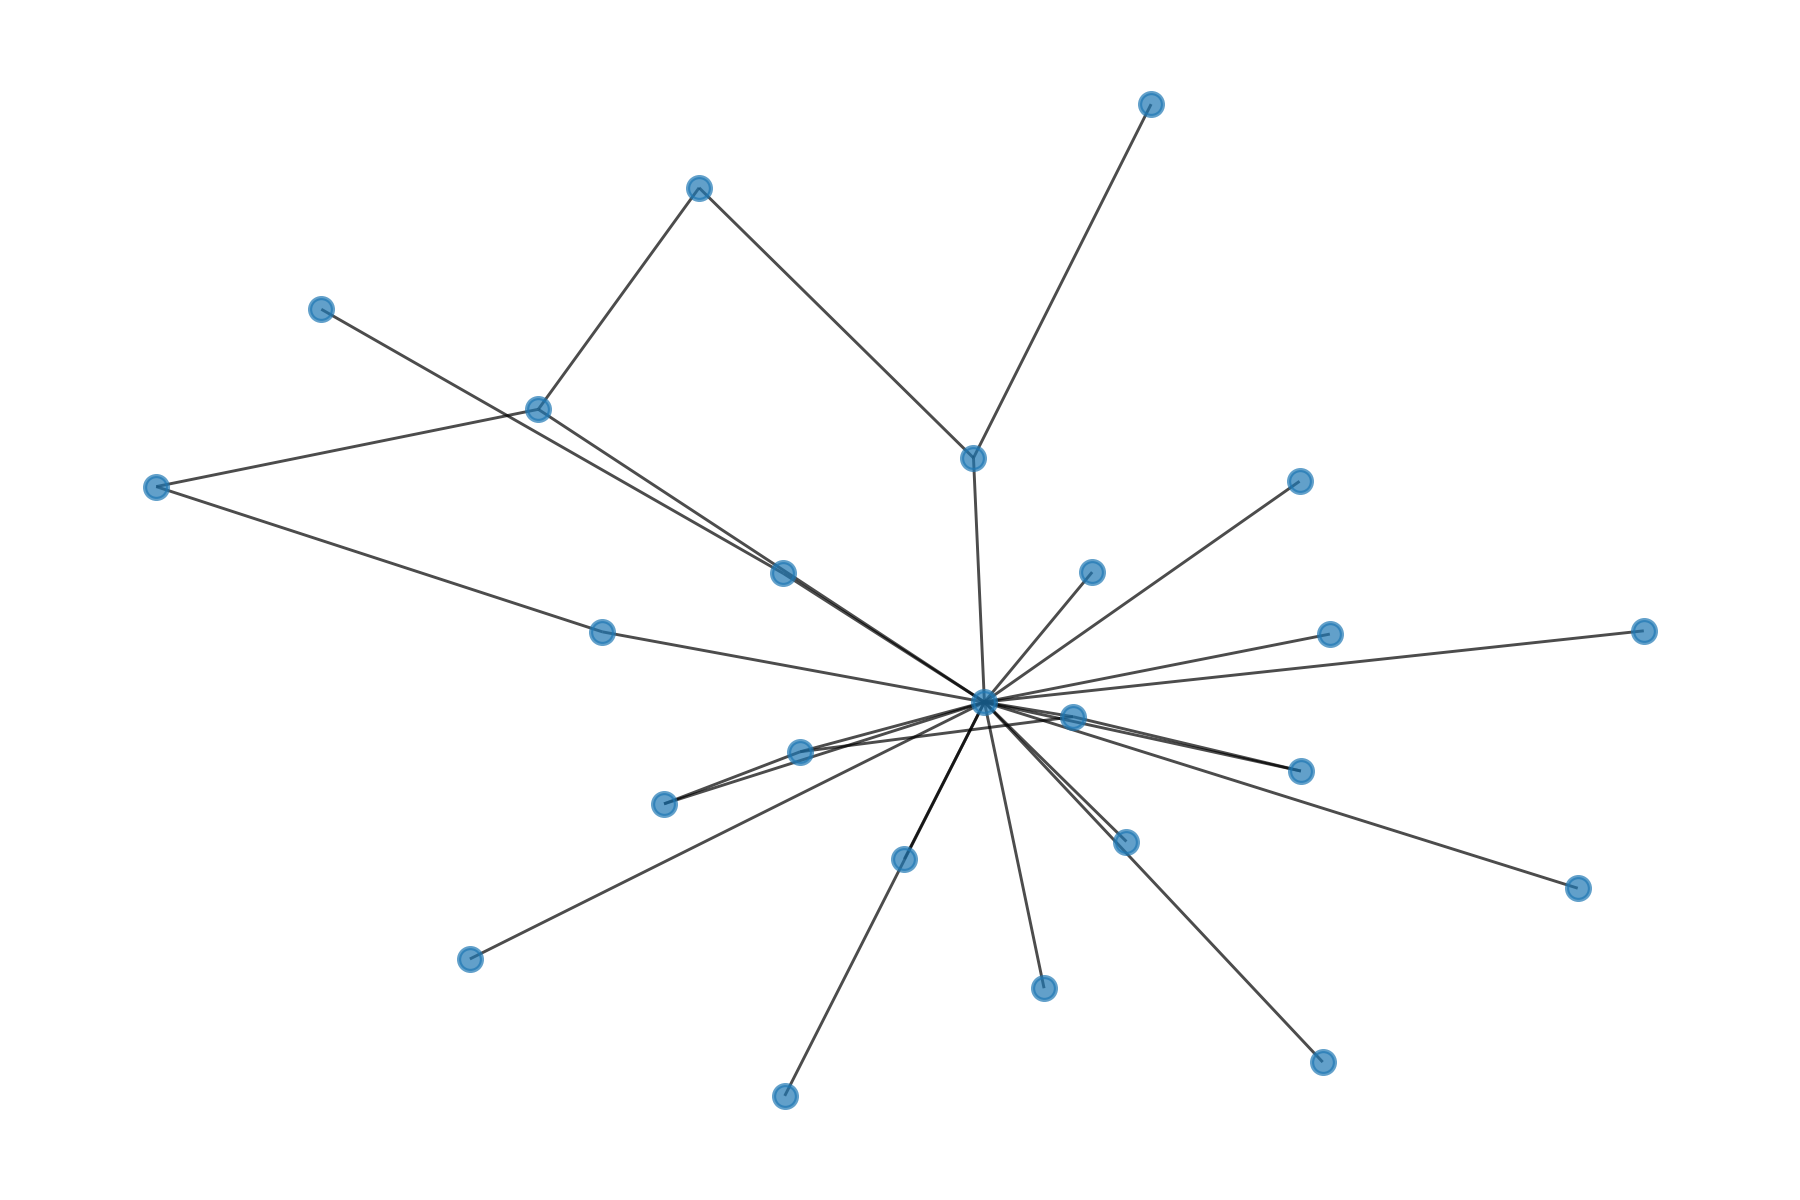
\includegraphics[width=1\linewidth]{problem_02/network_phase2}
	\end{minipage}
	\begin{minipage}{.24\textwidth}
		\centering
		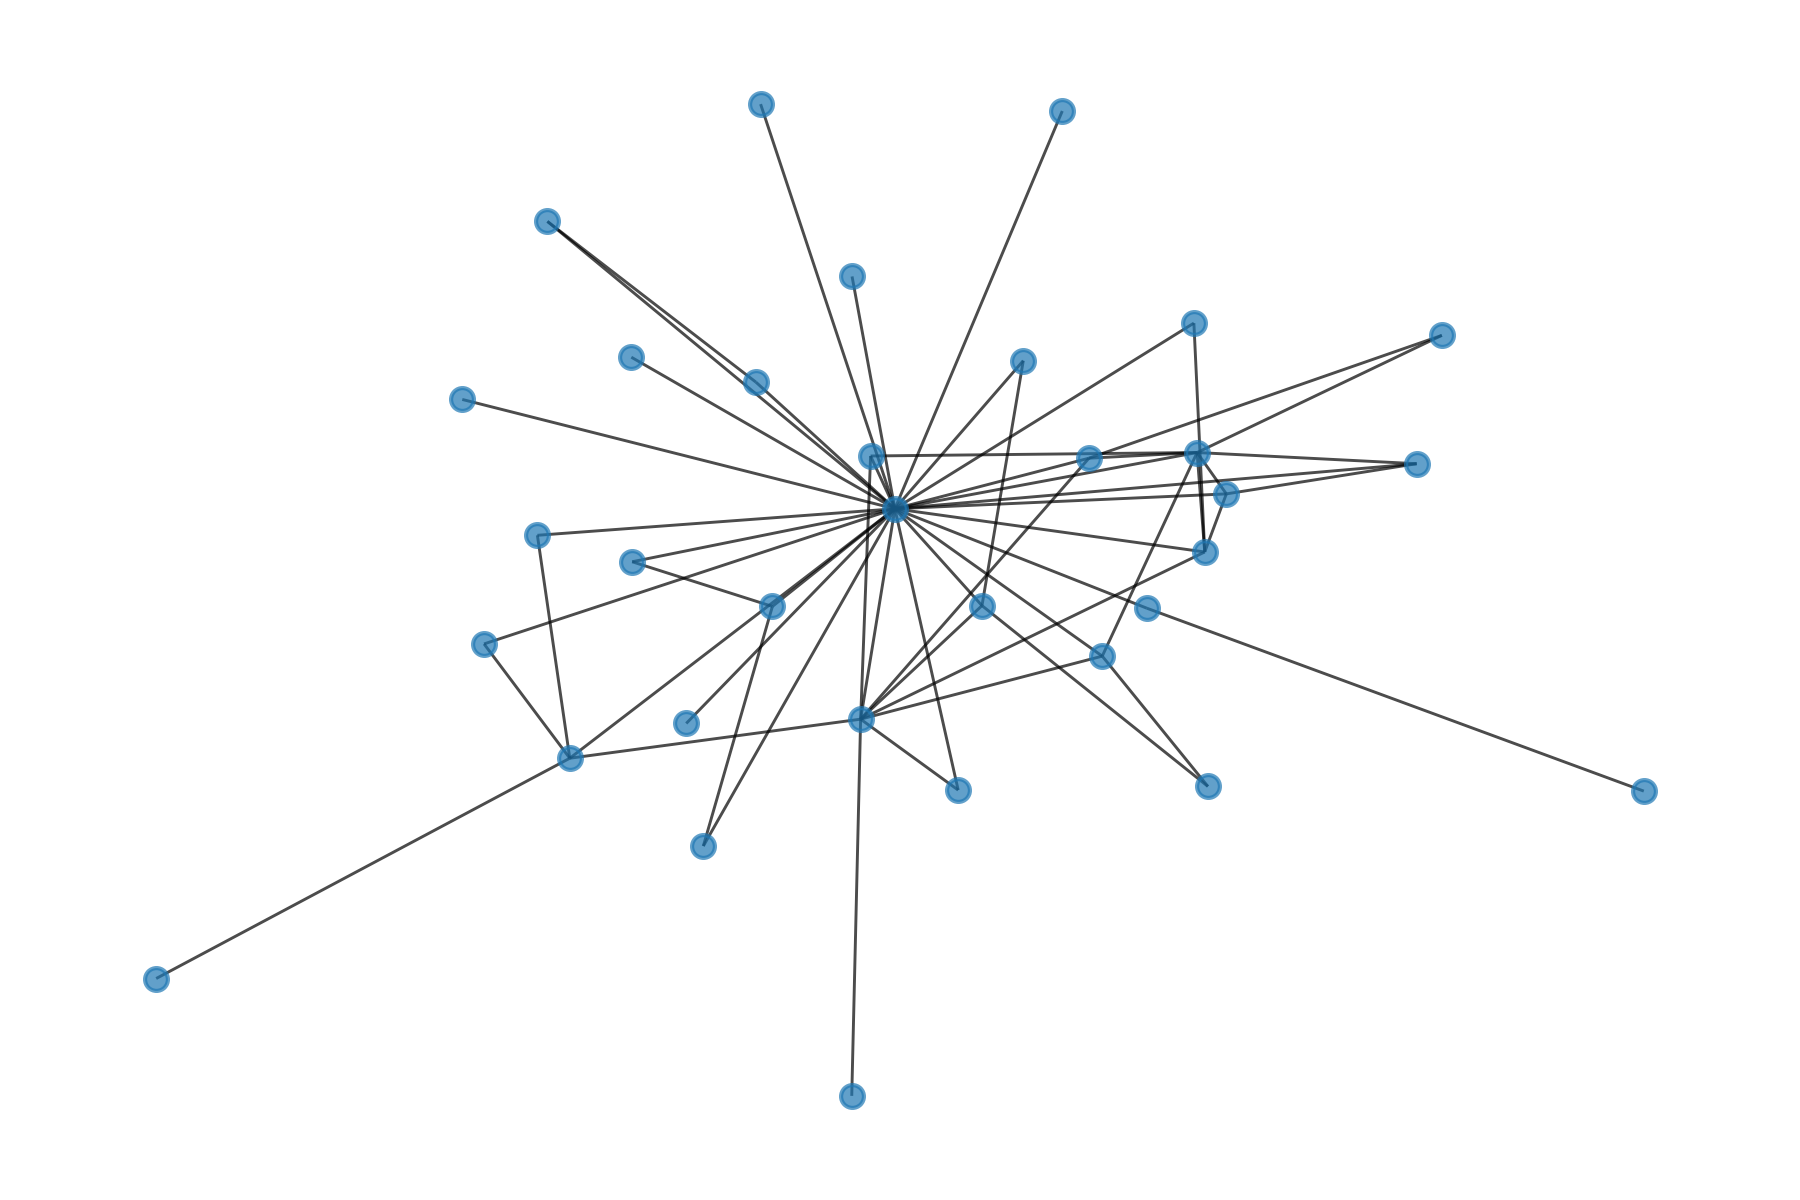
\includegraphics[width=1\linewidth]{problem_02/network_phase3}
	\end{minipage}
	\begin{minipage}{.24\textwidth}
		\centering
		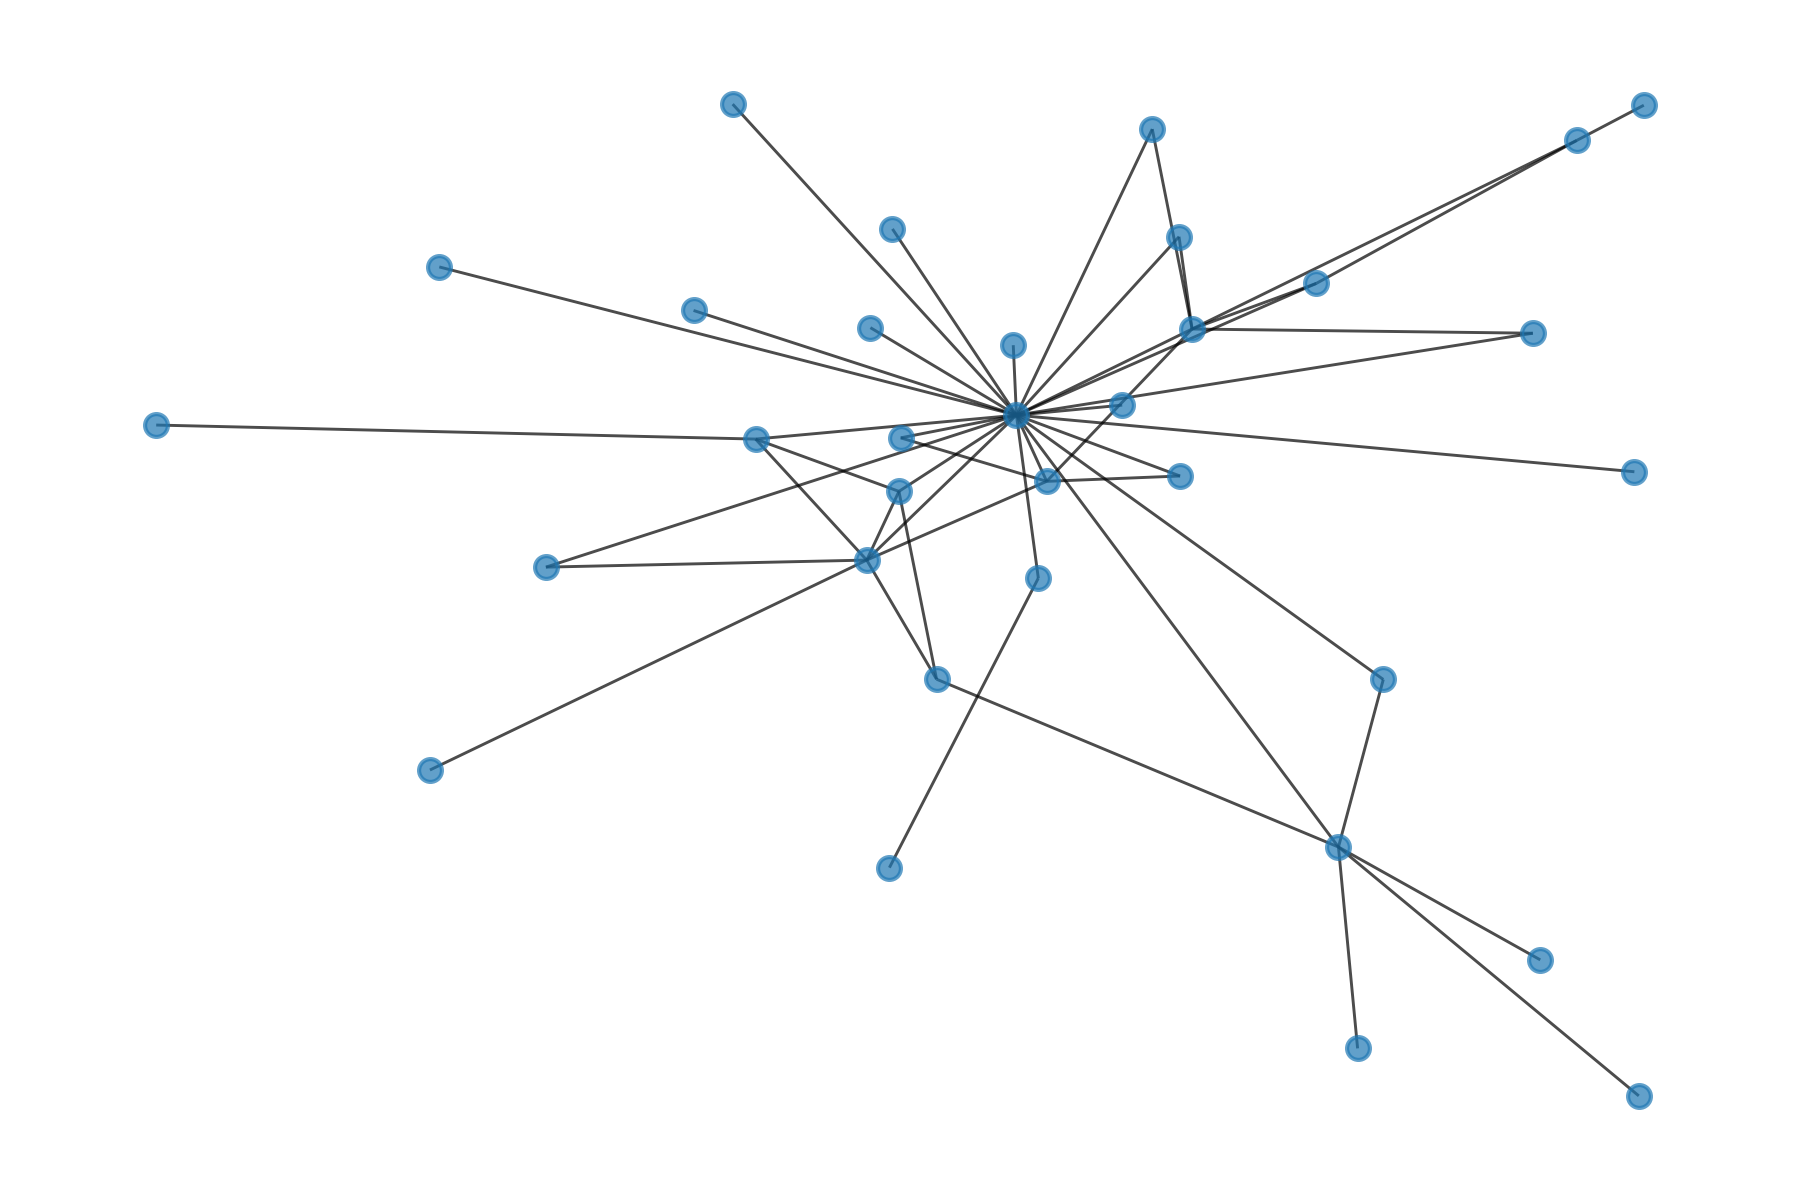
\includegraphics[width=1\linewidth]{problem_02/network_phase4}
	\end{minipage}
		\begin{minipage}{.24\textwidth}
		\centering
		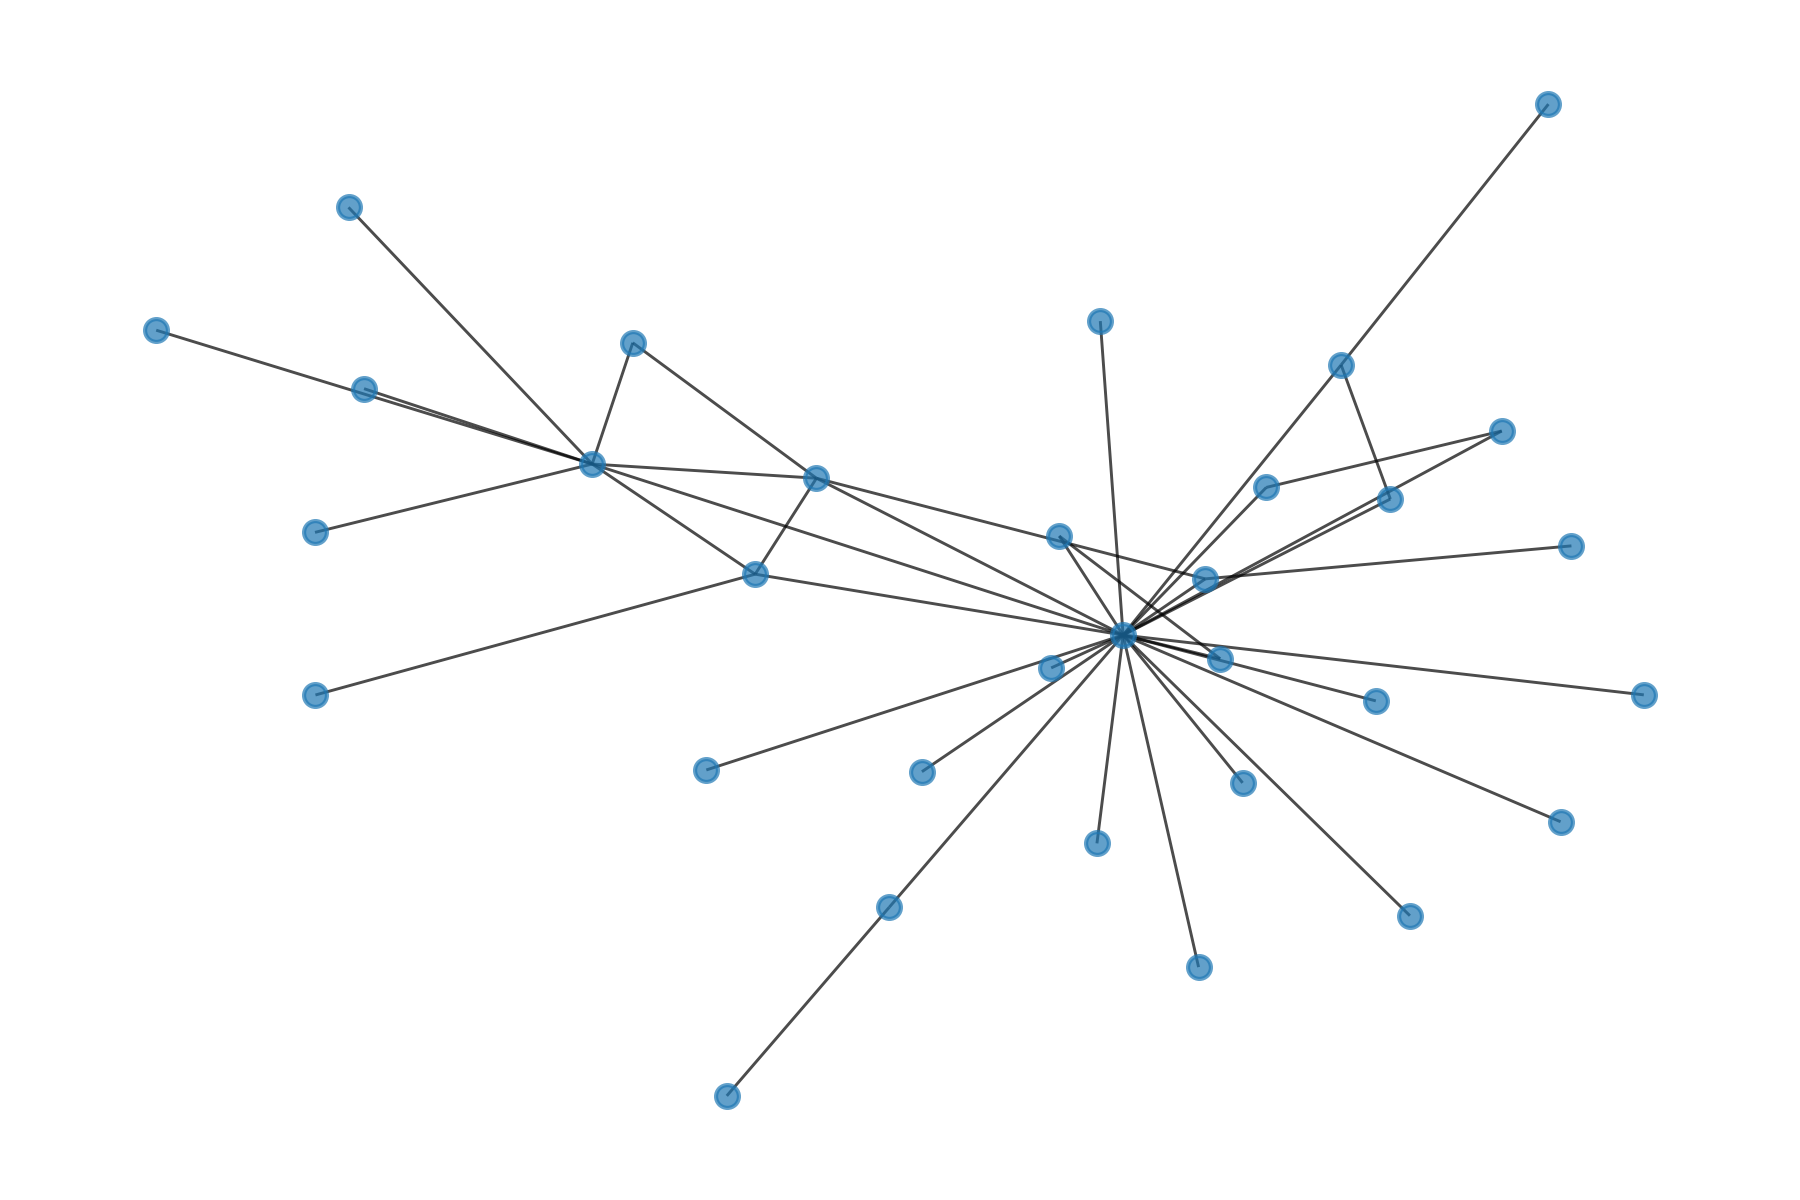
\includegraphics[width=1\linewidth]{problem_02/network_phase5}
	\end{minipage}
	\begin{minipage}{.24\textwidth}
		\centering
		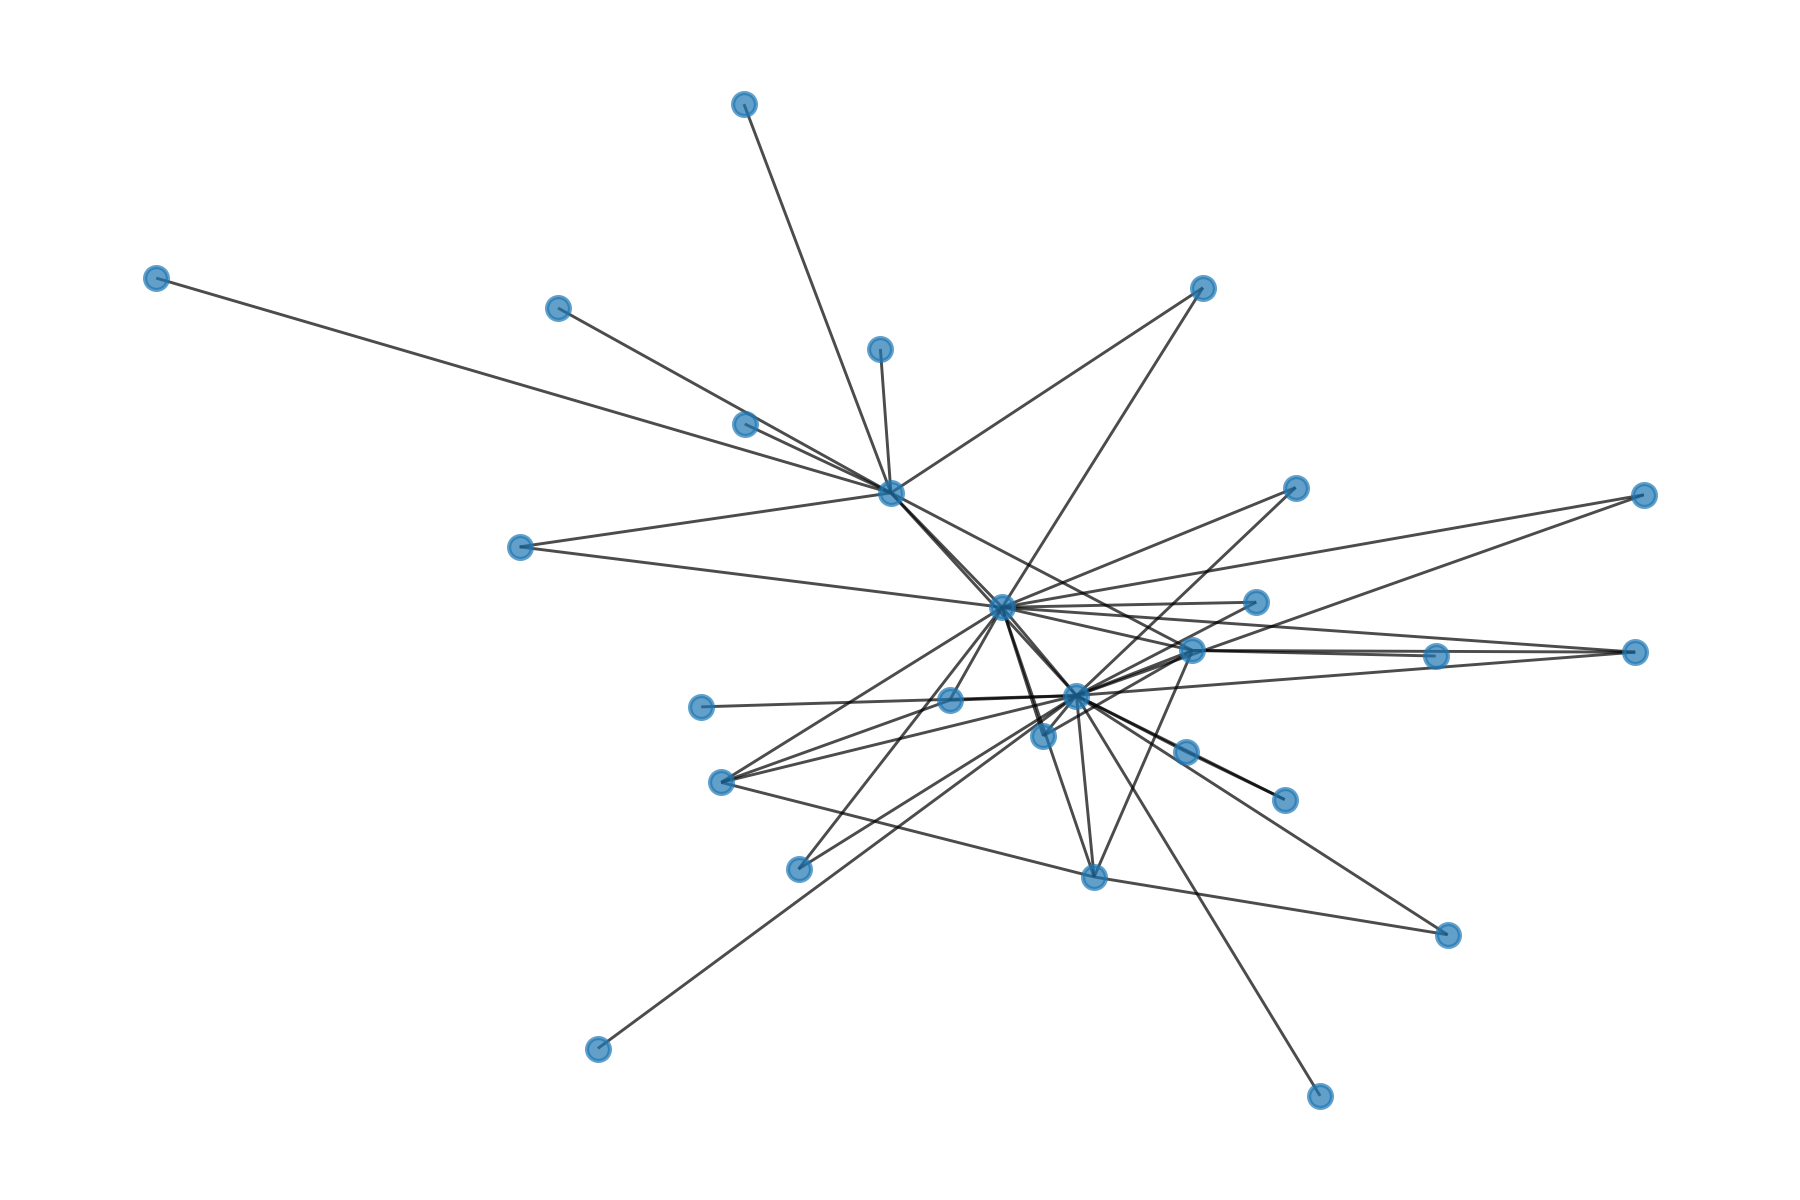
\includegraphics[width=1\linewidth]{problem_02/network_phase6}
	\end{minipage}
	\begin{minipage}{.24\textwidth}
		\centering
		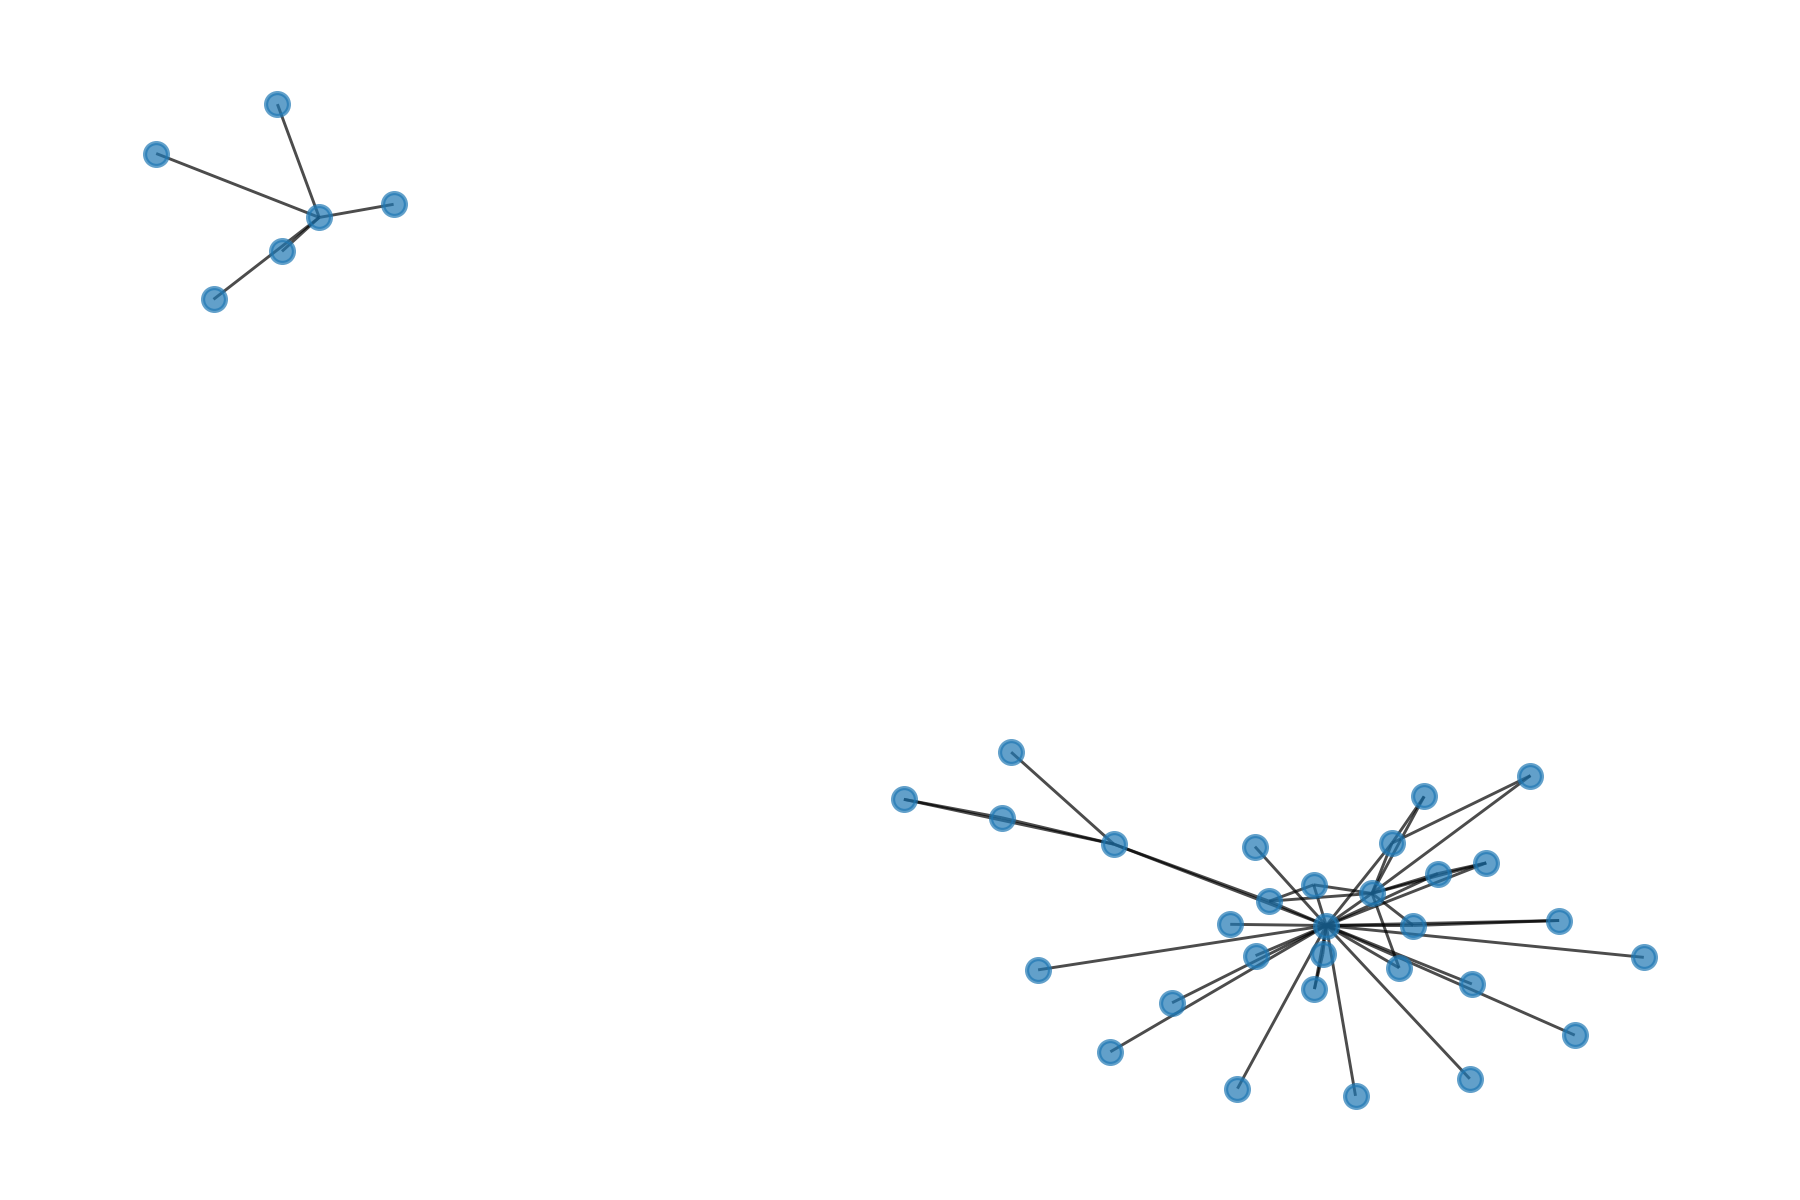
\includegraphics[width=1\linewidth]{problem_02/network_phase7}
	\end{minipage}
	\begin{minipage}{.24\textwidth}
		\centering
		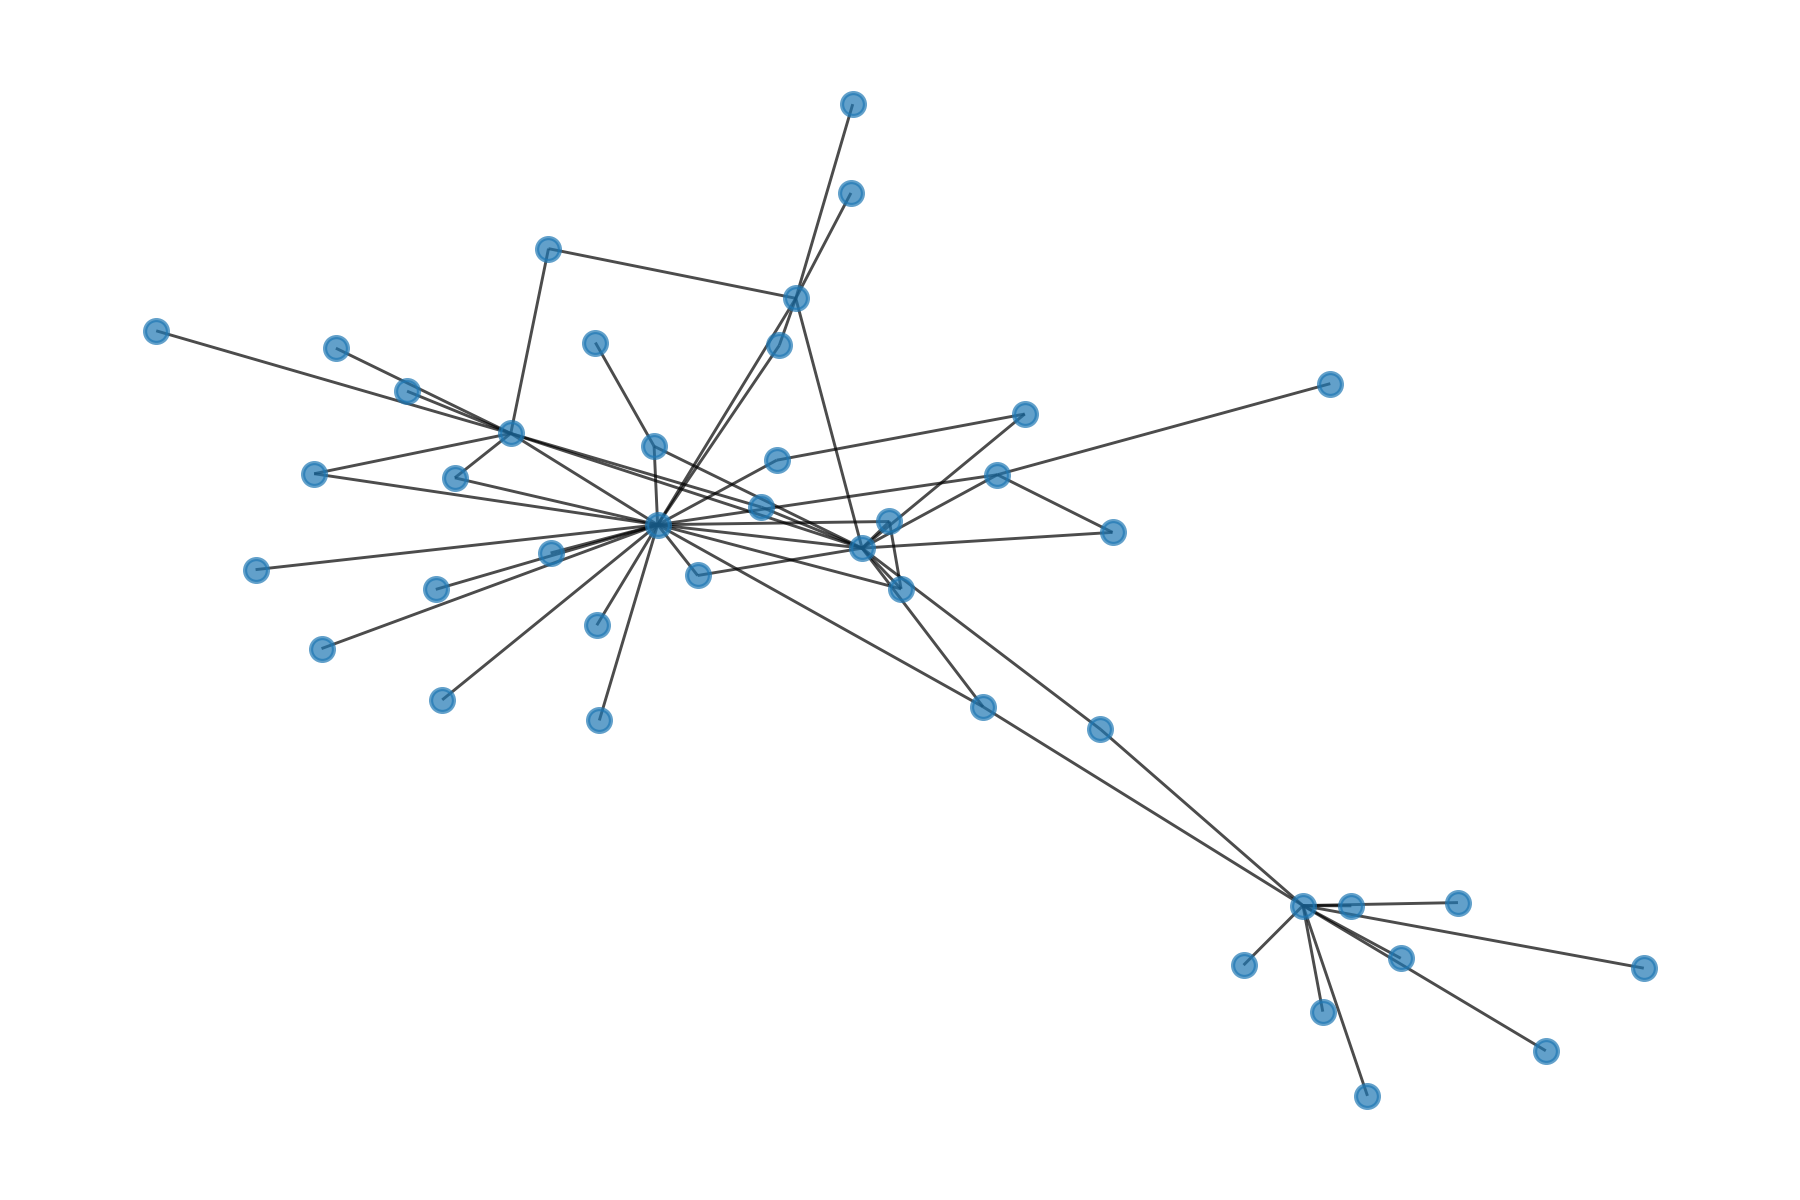
\includegraphics[width=1\linewidth]{problem_02/network_phase8}
	\end{minipage}
	\begin{minipage}{.24\textwidth}
		\centering
		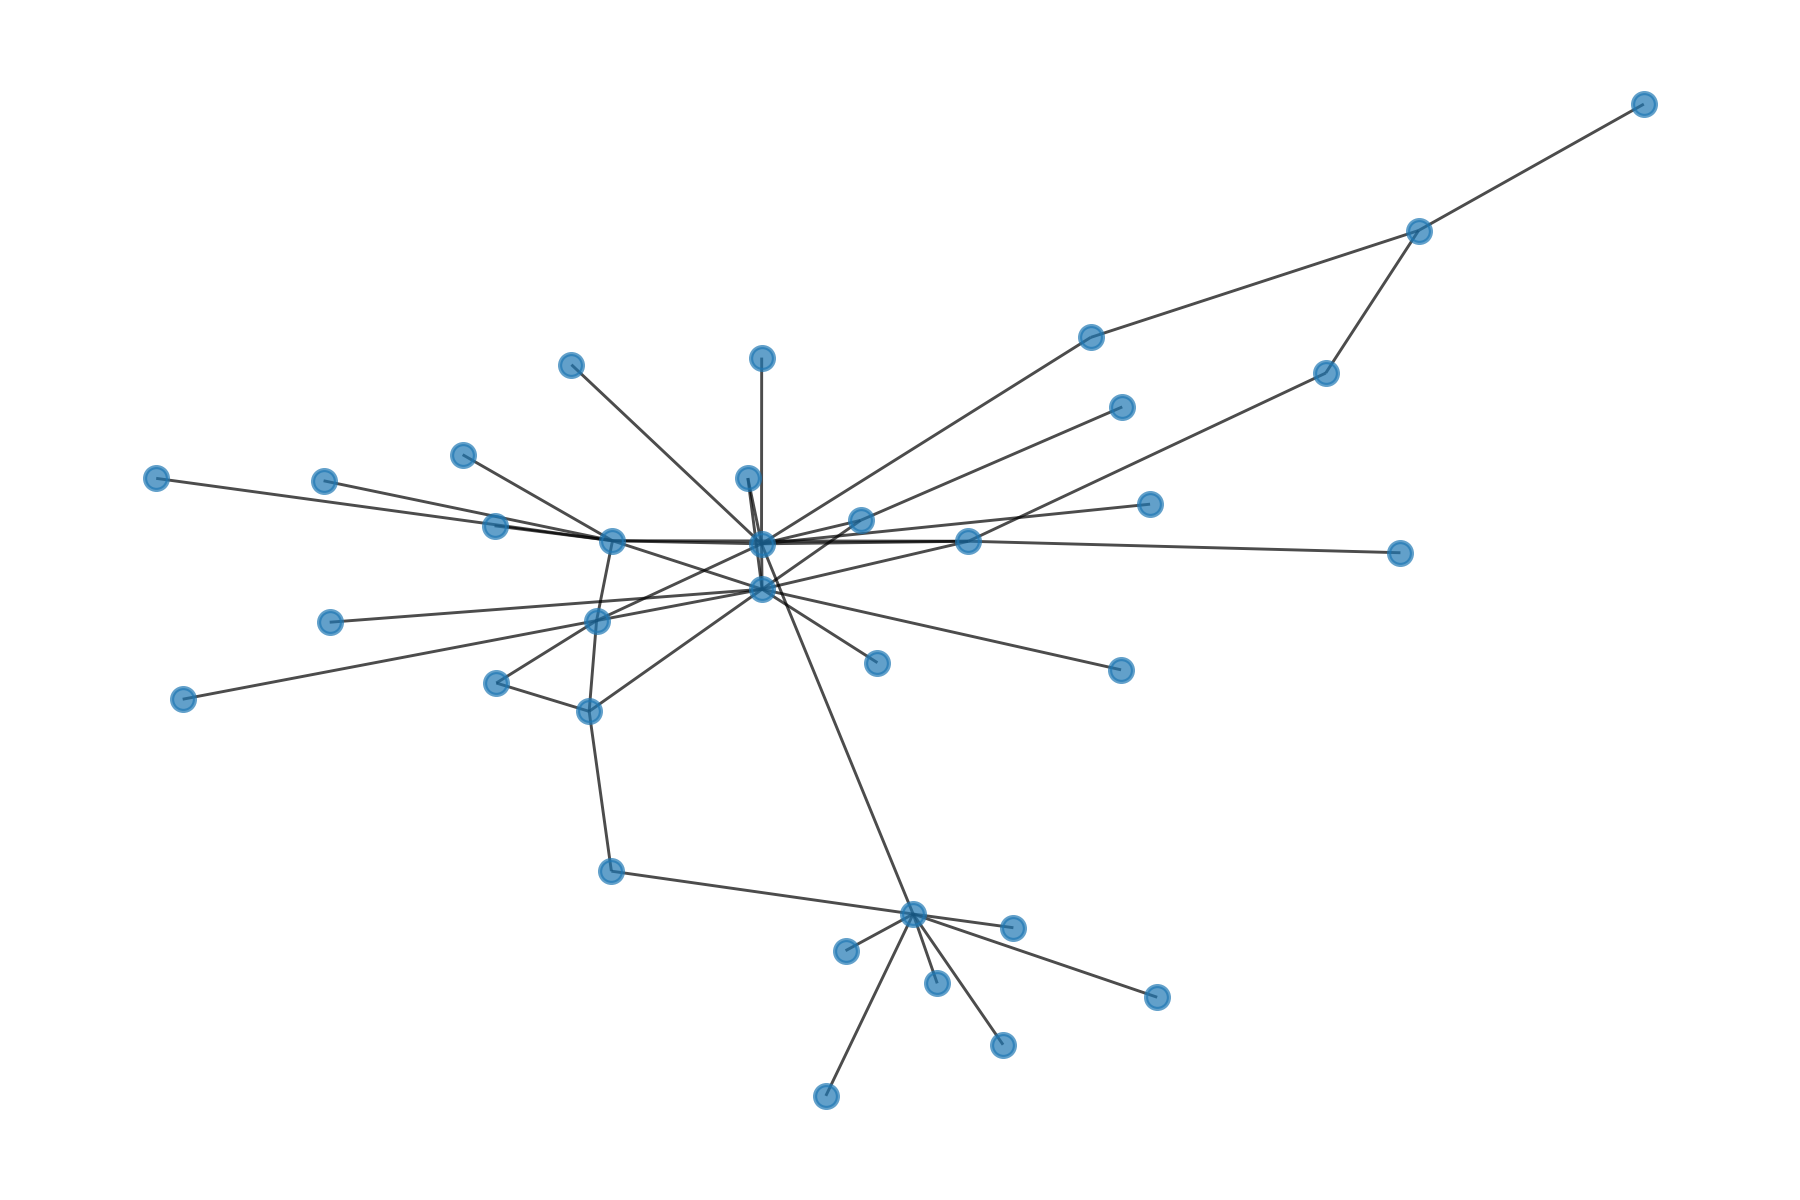
\includegraphics[width=1\linewidth]{problem_02/network_phase9}
	\end{minipage}
	\begin{minipage}{.24\textwidth}
		\centering
		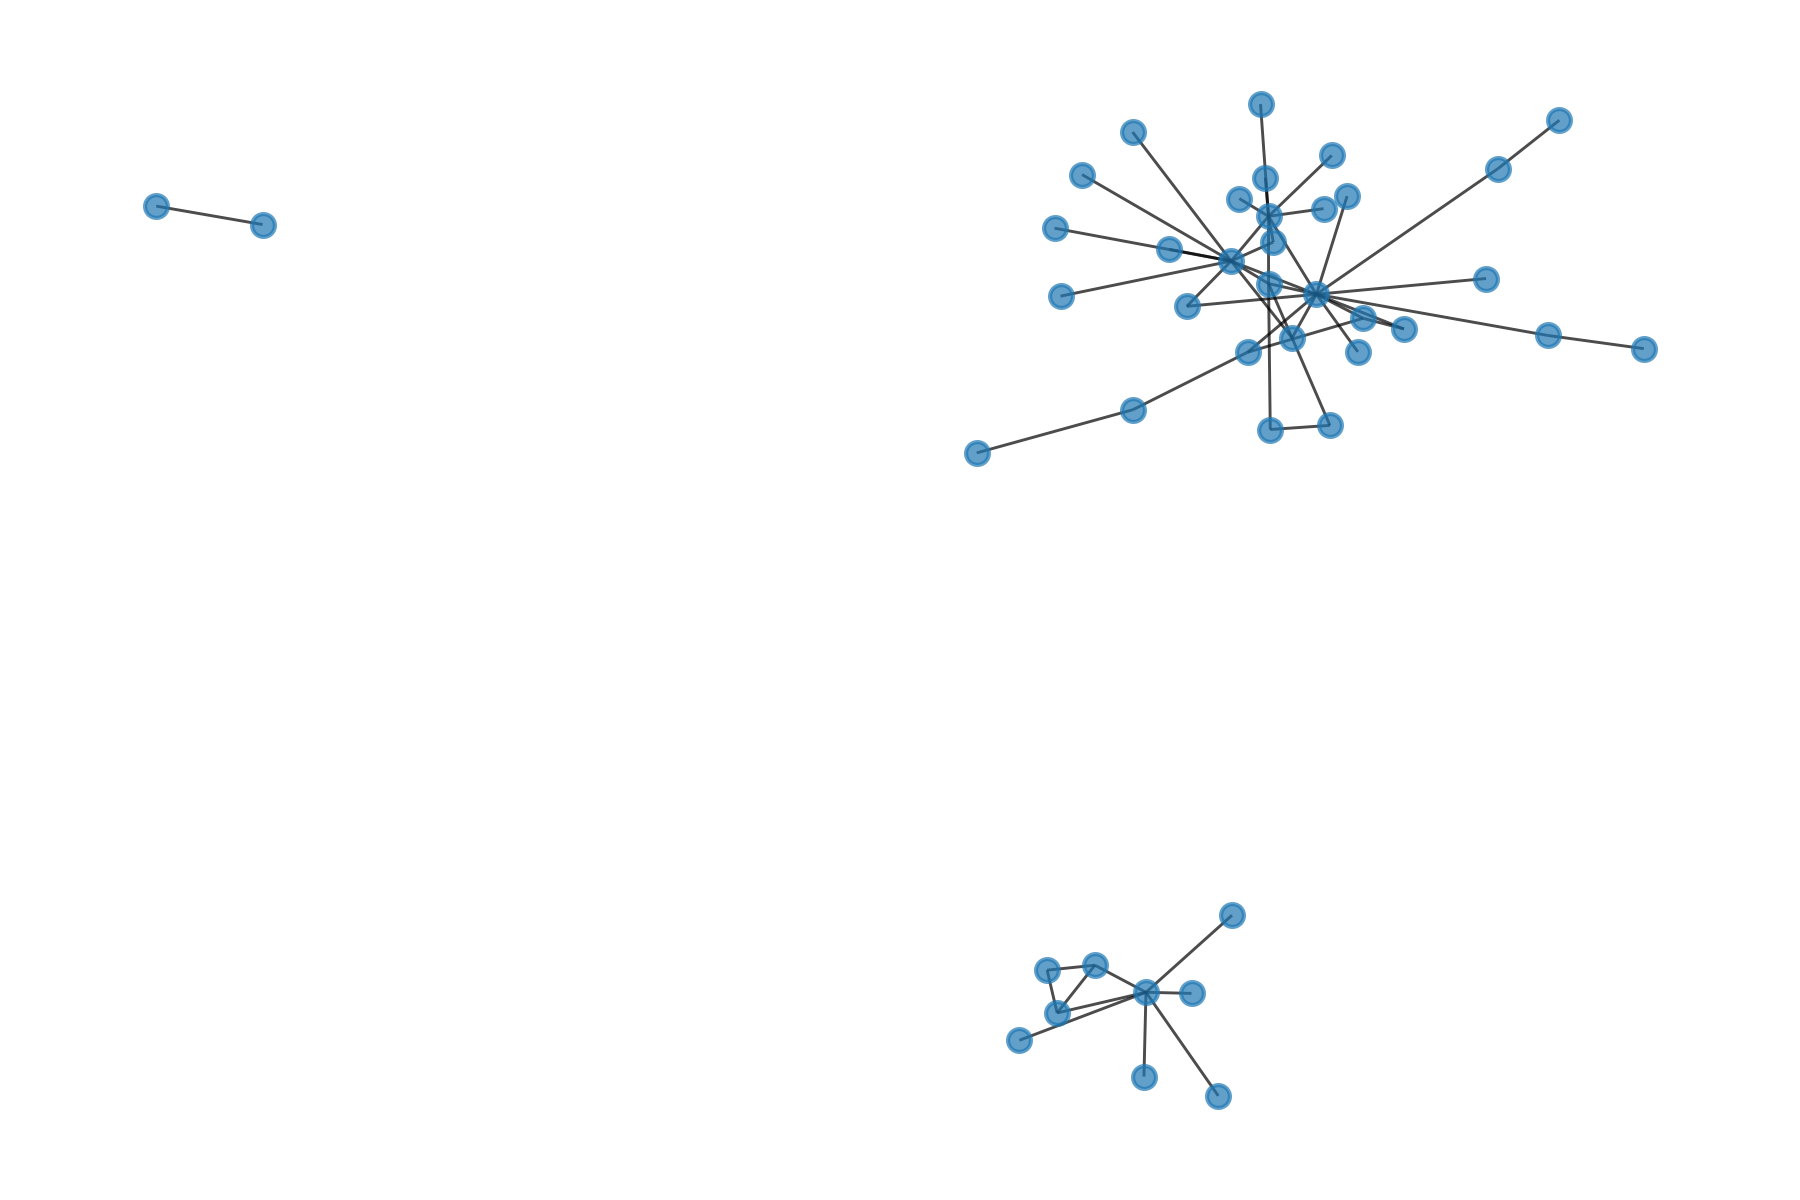
\includegraphics[width=1\linewidth]{problem_02/network_phase10}
	\end{minipage}
	\begin{minipage}{.24\textwidth}
		\centering
		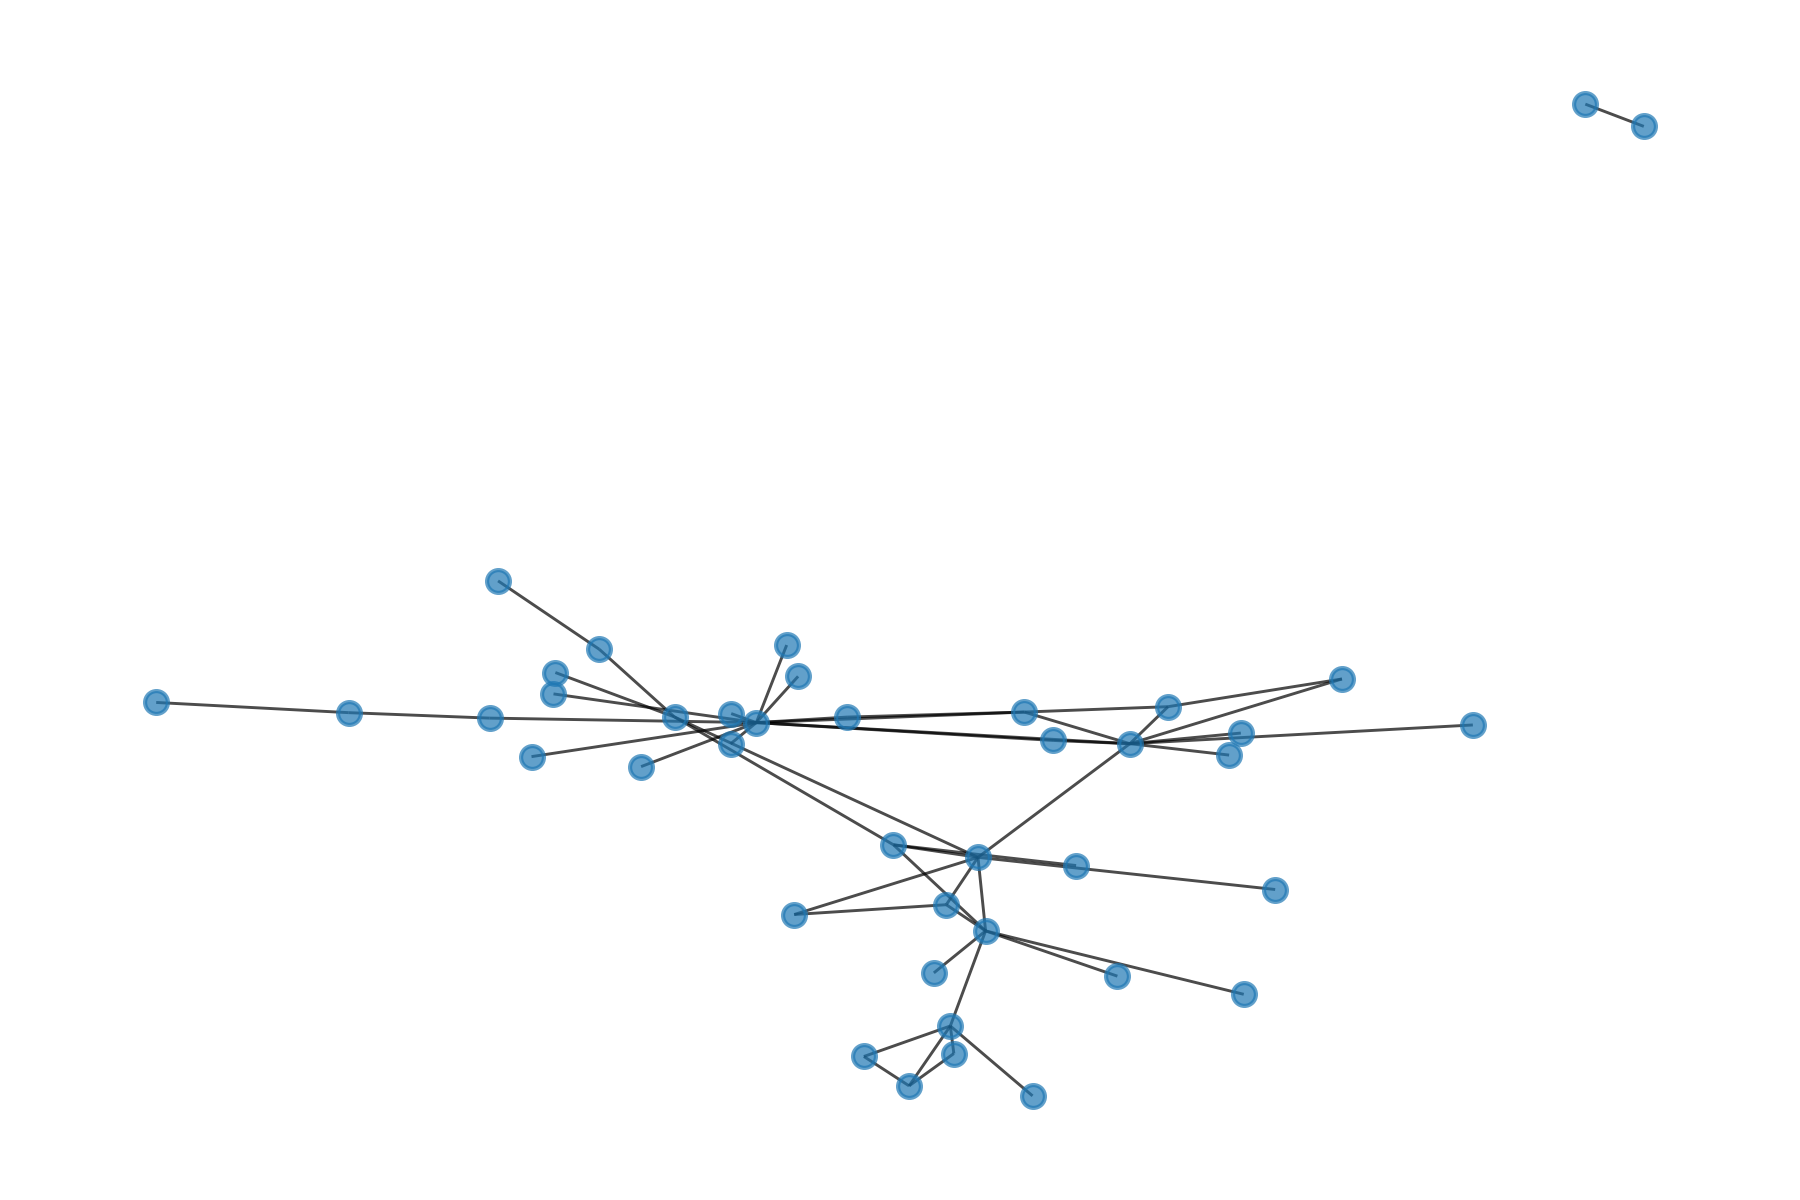
\includegraphics[width=1\linewidth]{problem_02/network_phase11}
	\end{minipage}
	\caption{CAVIAR network visualization over different phases (from left to right, from top to bottom: phase 1,..., phase 11, without node labels)}
	\label{fig:network_visualization}
\end{figure}

\begin{figure}[htbp]
	\centering
	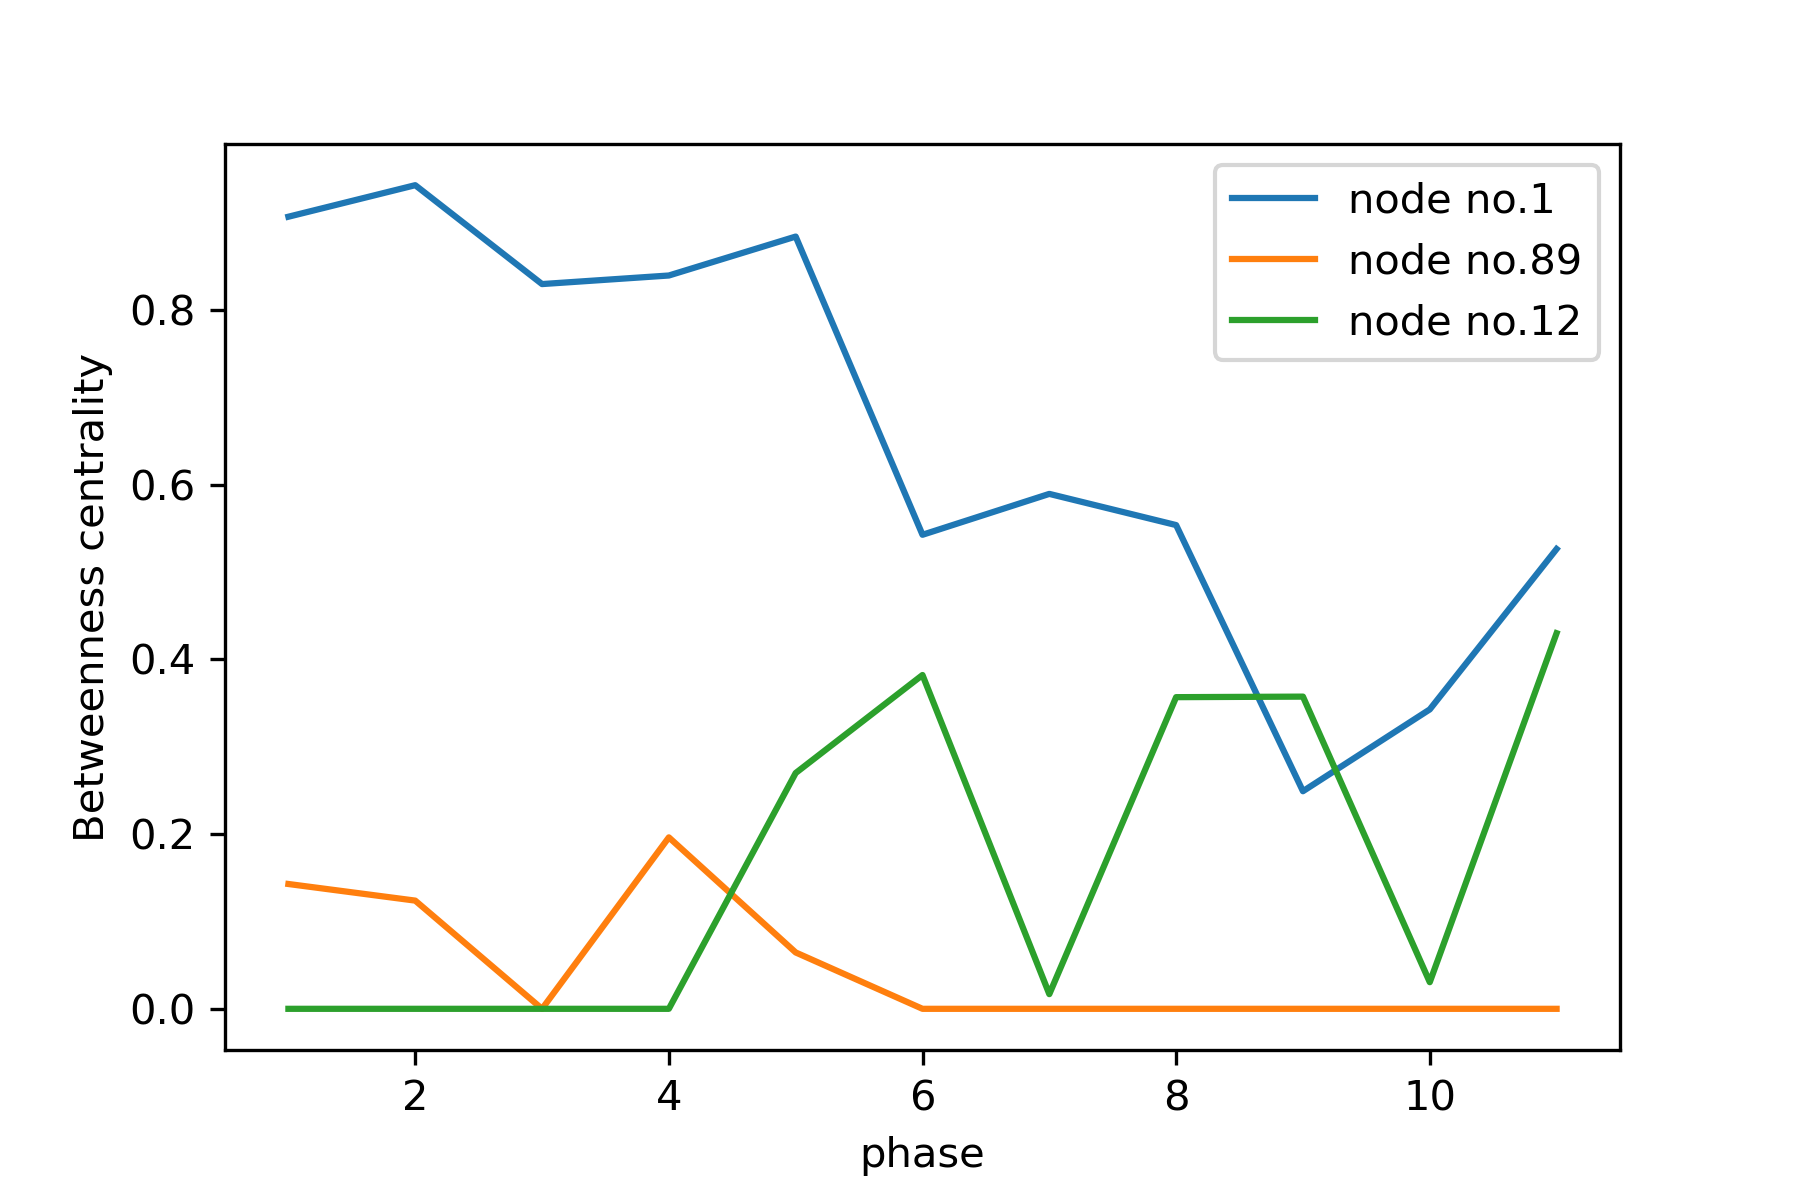
\includegraphics[width=0.7\linewidth]{problem_02/betweenness_specific_nodes}
	\caption{Betweenness centrality of specific nodes over phases}
	\label{fig:betweenness_specific_nodes}
\end{figure}

There are some interesting shifts in the development to see at phases 3-4-5 and phases 8-9-10. In the first period the network responds to a seizure of 300kg marijuana in value of 2.5x$10^6$\$ in phase 4 (see figure \ref{fig:visualization_phases_3_5_labels}). Here, the node no. 89 reaches its maximum importance according to betweenness centrality as node no. 1 stays on a high level between 0.8-0.9 (see figure \ref{fig:betweenness_specific_nodes}).\\

\begin{figure}[htbp]
	\centering
	\begin{minipage}{.32\textwidth}
		\centering
		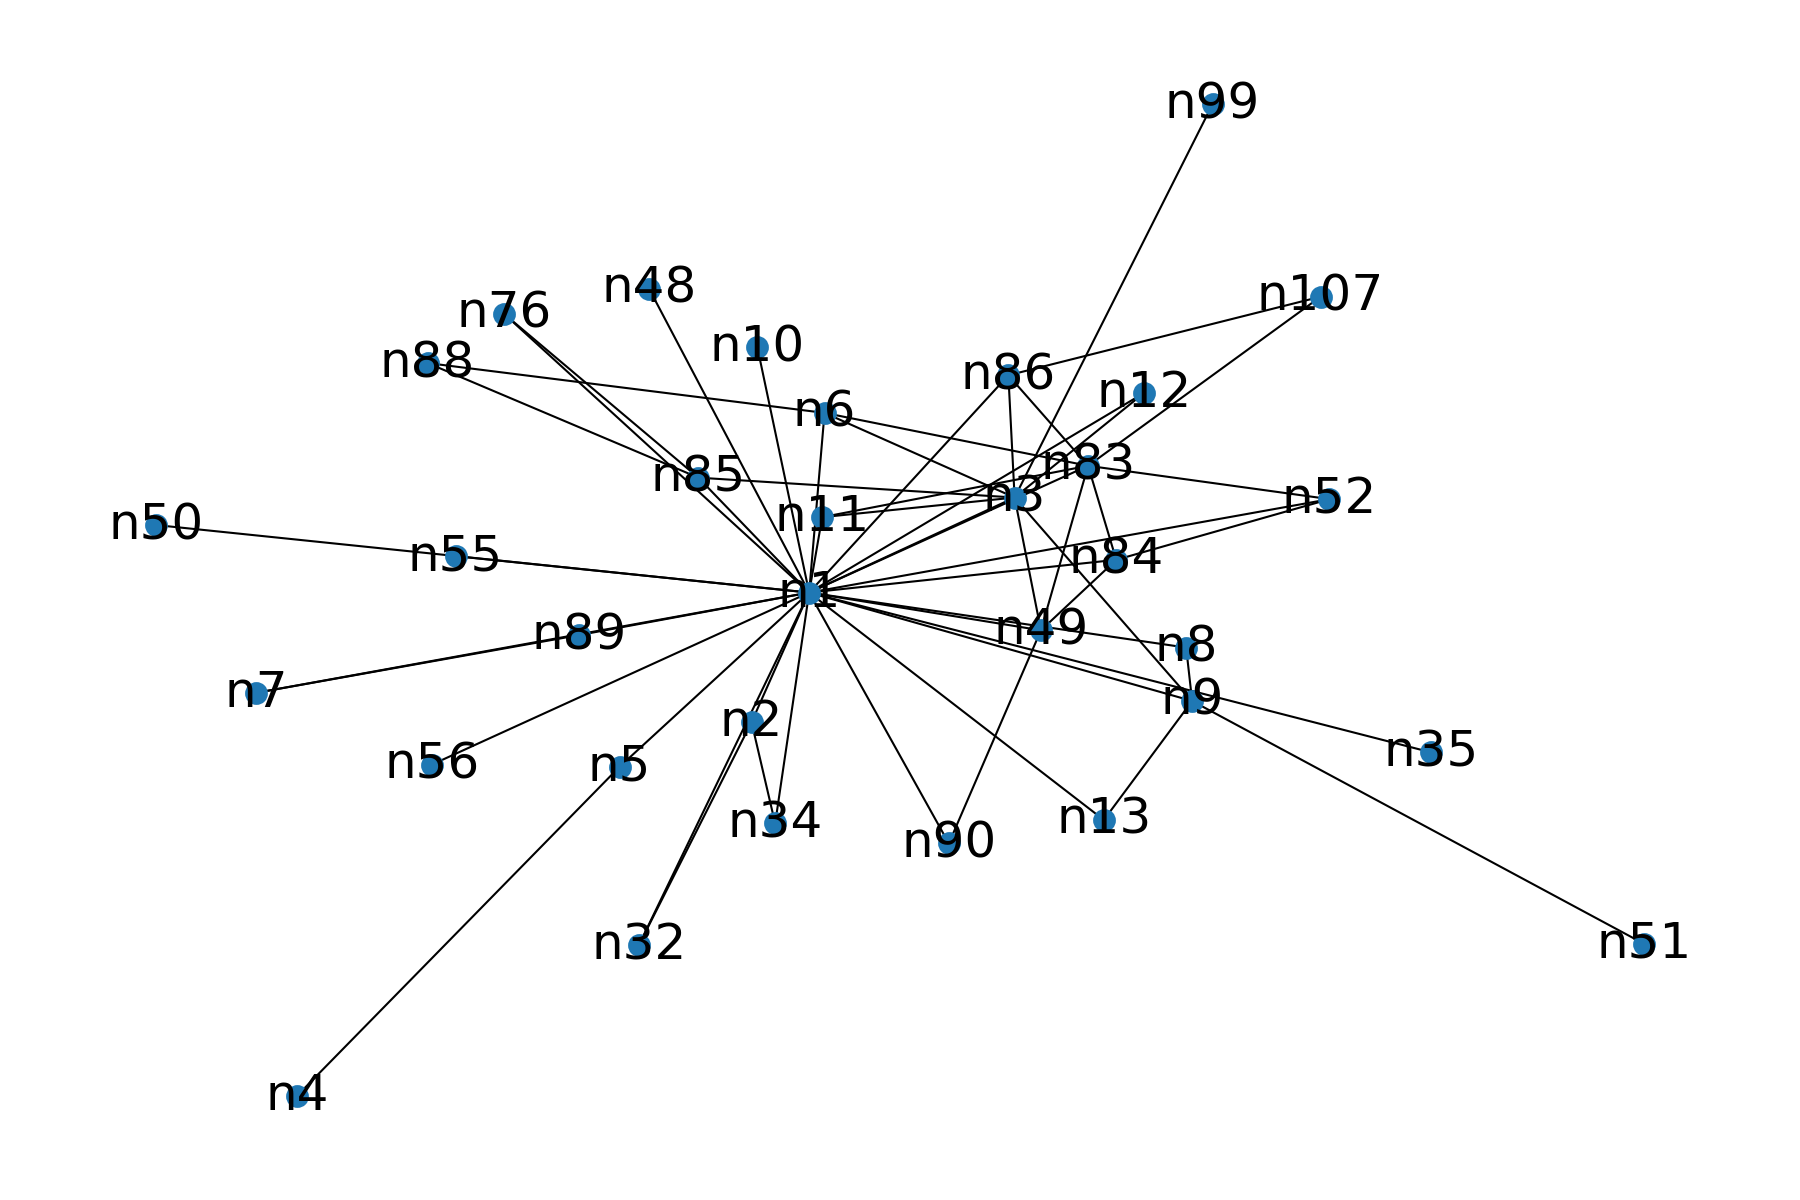
\includegraphics[width=1\linewidth]{problem_02/network_labels_phase3}
	\end{minipage}
	\begin{minipage}{.32\textwidth}
		\centering
		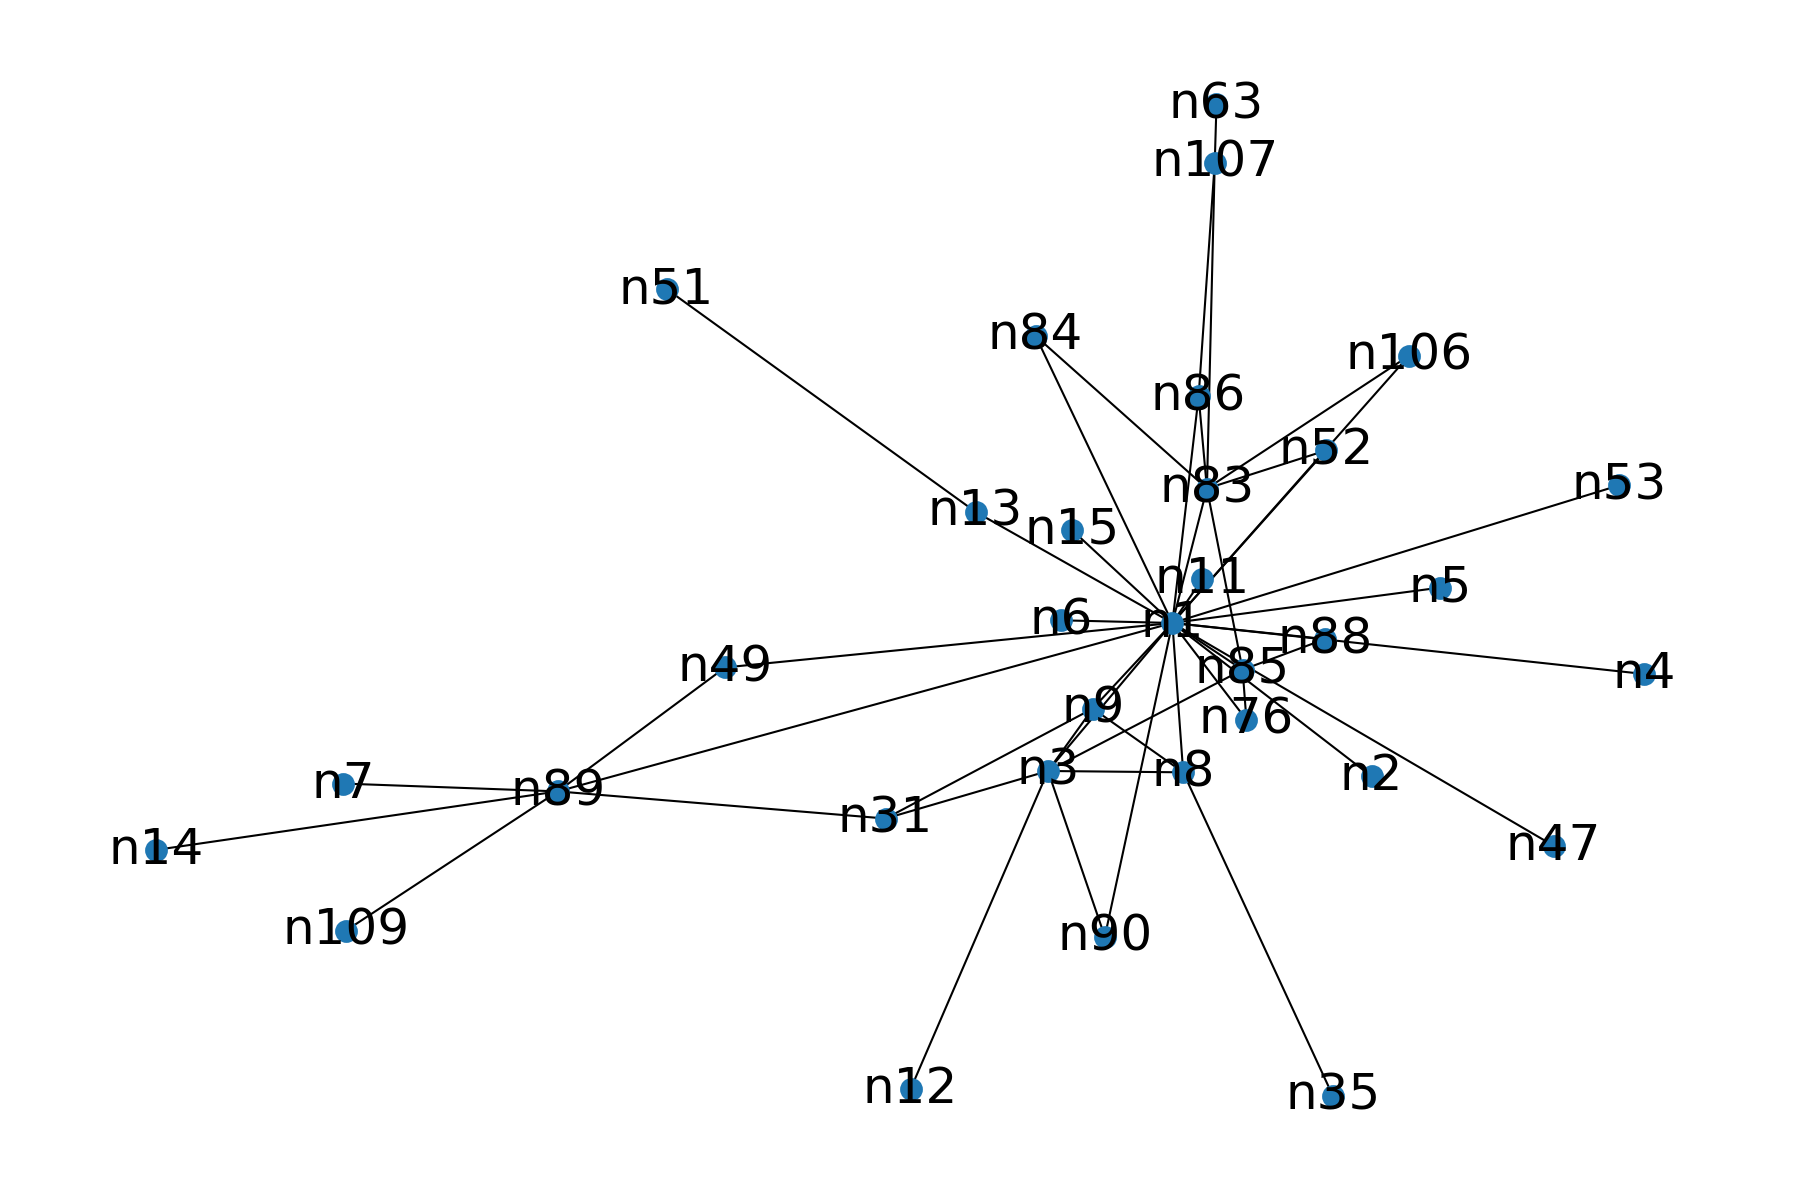
\includegraphics[width=1\linewidth]{problem_02/network_labels_phase4}
	\end{minipage}
	\begin{minipage}{.32\textwidth}
		\centering
		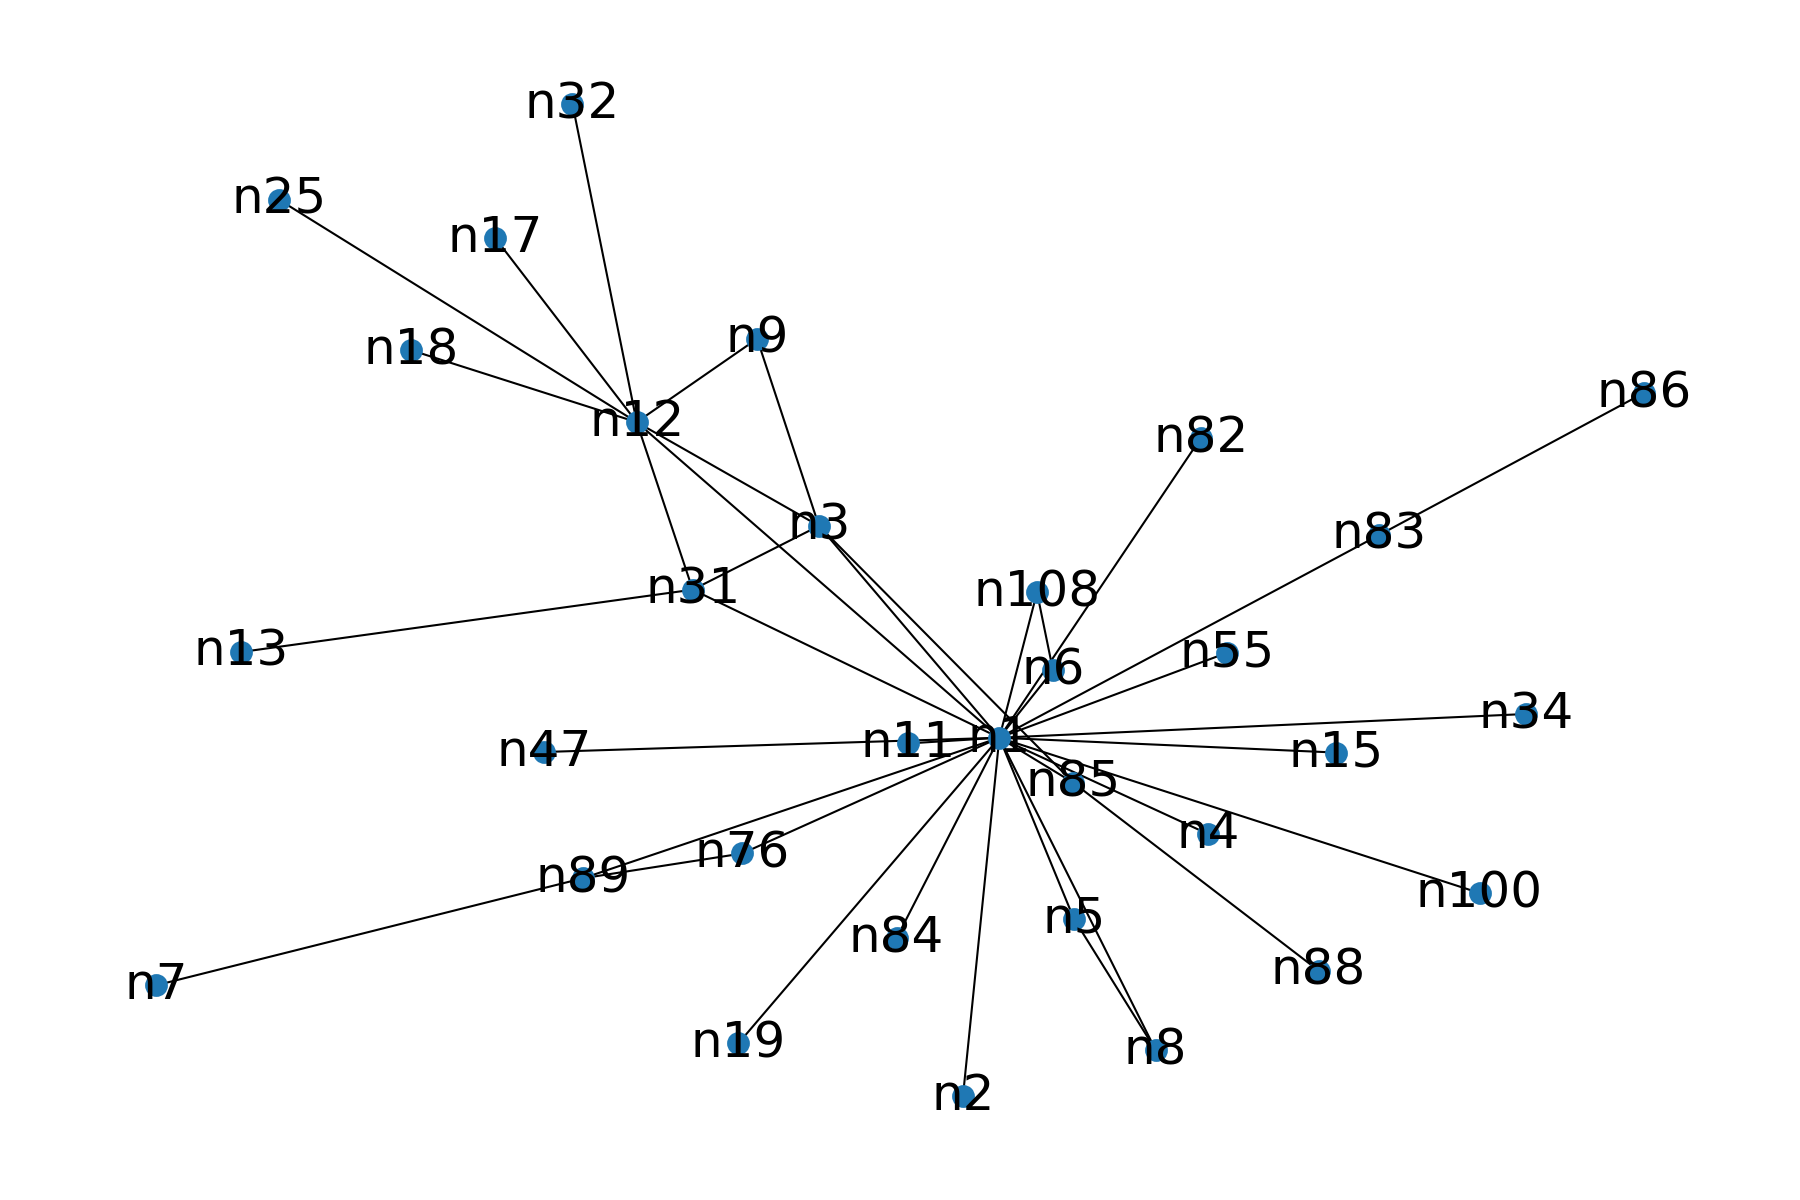
\includegraphics[width=1\linewidth]{problem_02/network_labels_phase5}
	\end{minipage}
	\caption{CAVIAR network visualization over different phases (from left to right: phase 3, phase 4, phase 5, with node labels)}
\label{fig:visualization_phases_3_5_labels}
\end{figure}

The second period around the phases 8, 9 and 10 is significant as well (see figure \ref{fig:visualization_phases_8_10_labels}). Here, multiple seizures were done: Cocaine in value of 360x$10^3$\$ (phase 8) and cocaine and marijuana in total value of 4.3x$10^6$\$ (phase 9). This is the period in which node no. 1 reaches its minimum importance according to betweenness centrality whereas node no. 12 reaches its maximum (see figure \ref{fig:betweenness_specific_nodes}). In phase 10 node no. 12 is a central node for one separated small network.\\

\begin{figure}[htbp]
	\centering
	\begin{minipage}{.32\textwidth}
		\centering
		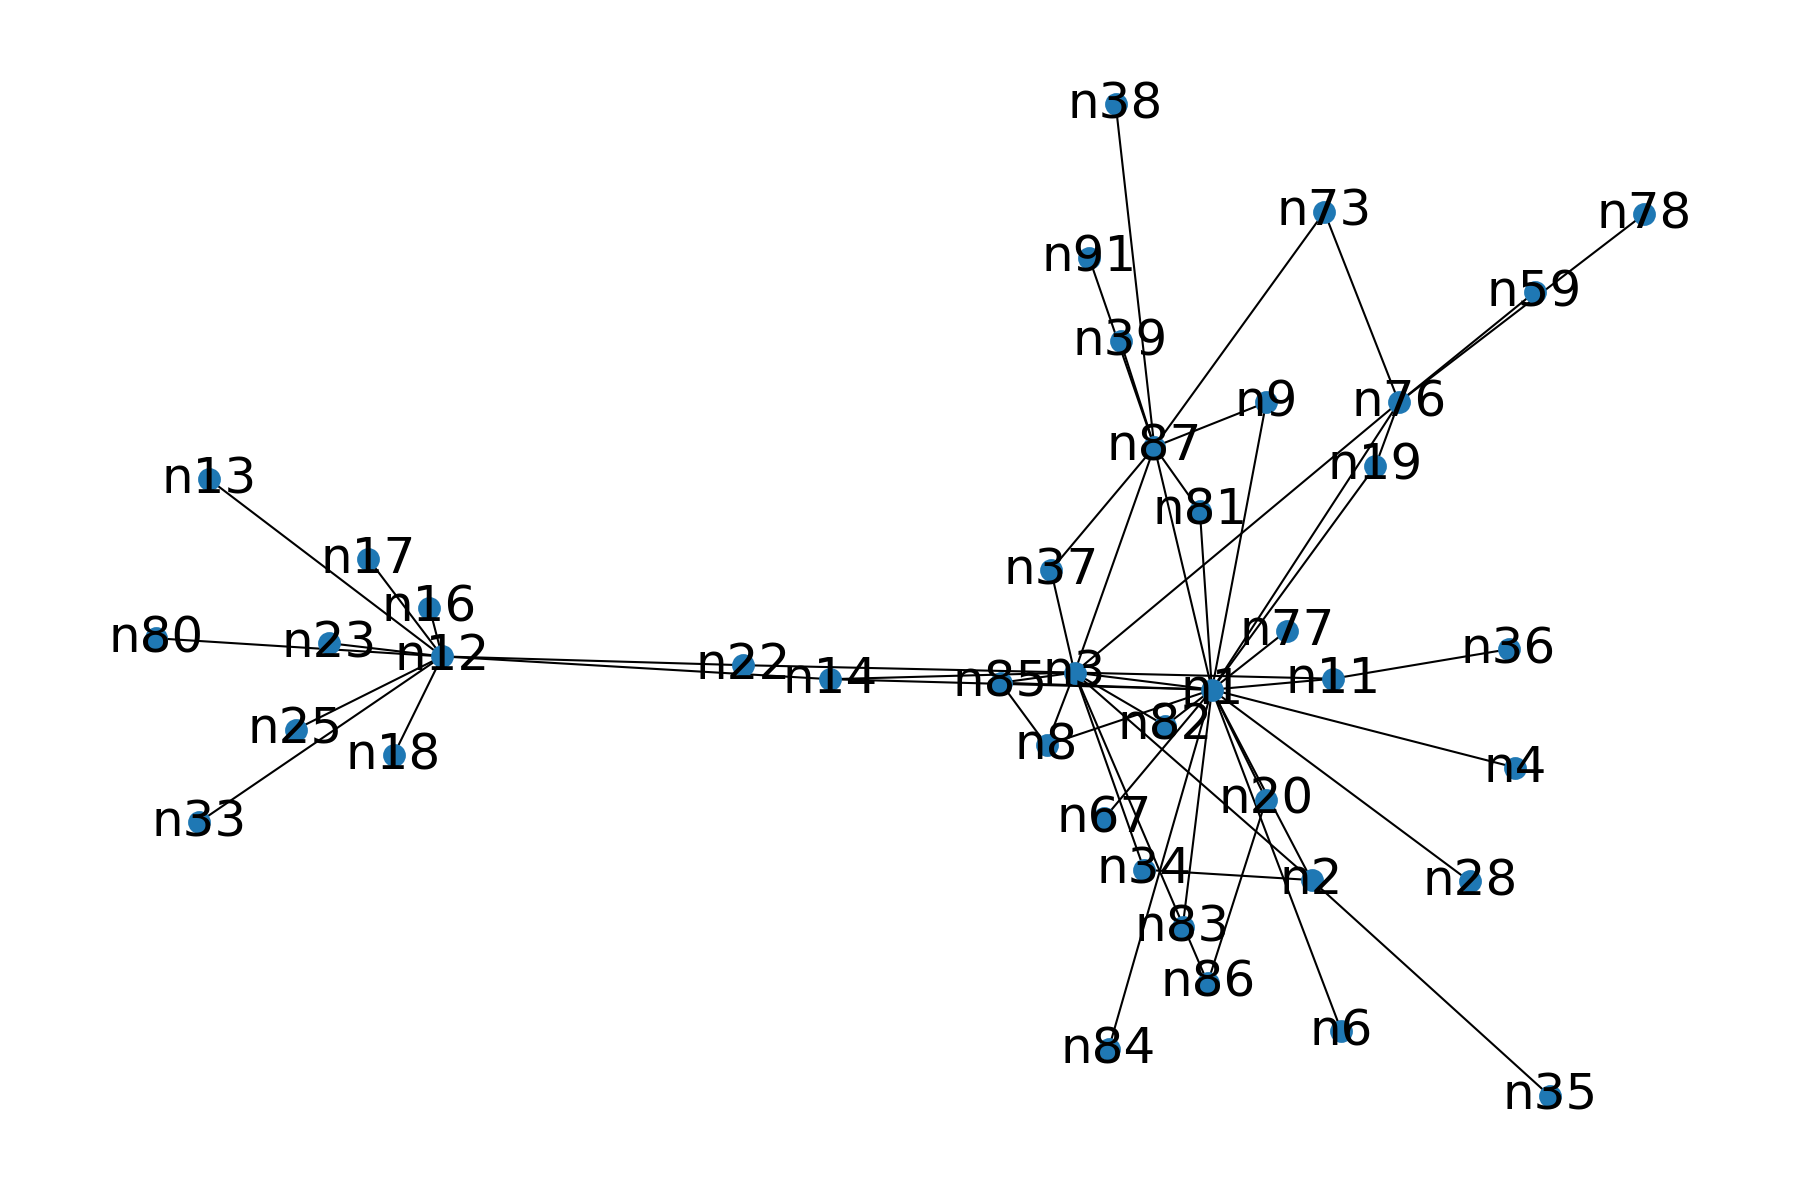
\includegraphics[width=1\linewidth]{problem_02/network_labels_phase8}
	\end{minipage}
	\begin{minipage}{.32\textwidth}
		\centering
		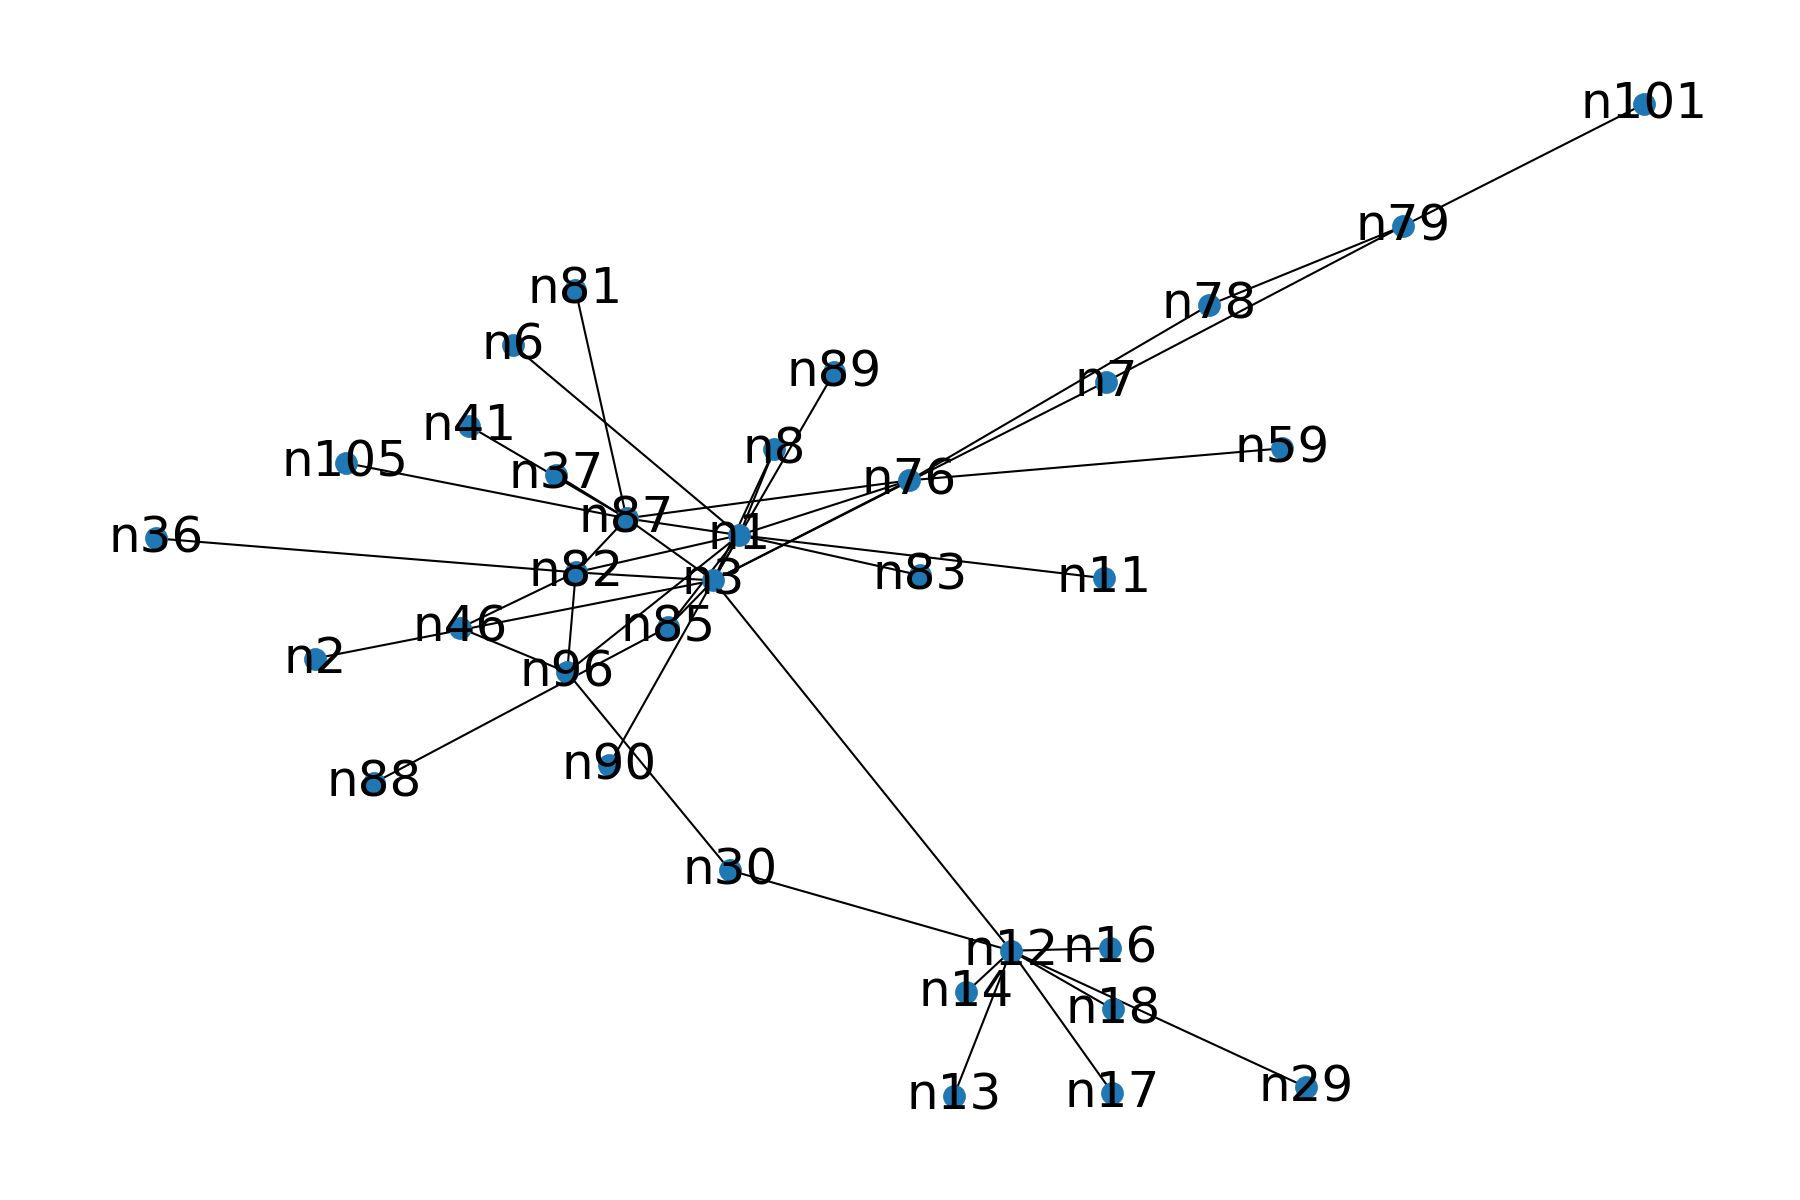
\includegraphics[width=1\linewidth]{problem_02/network_labels_phase9}
	\end{minipage}
	\begin{minipage}{.32\textwidth}
		\centering
		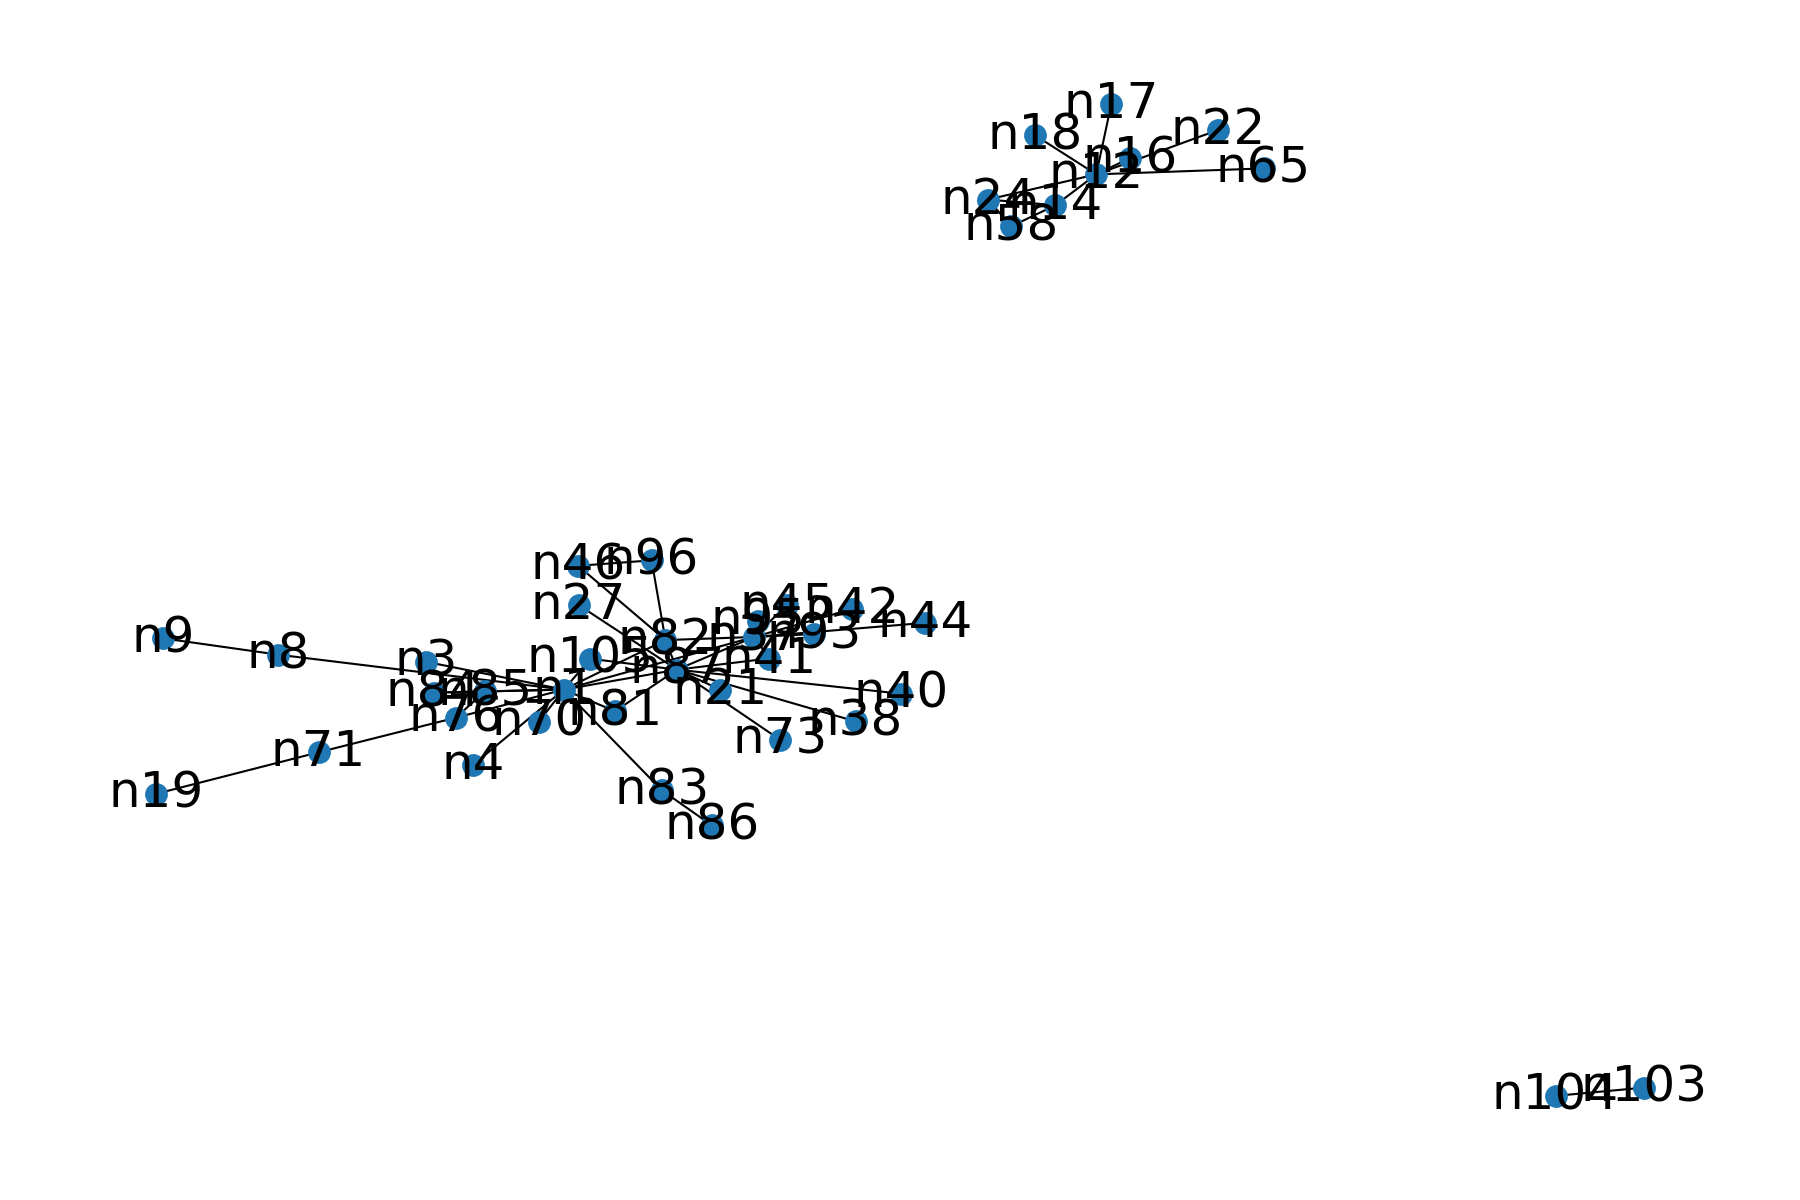
\includegraphics[width=1\linewidth]{problem_02/network_labels_phase10}
	\end{minipage}
	\caption{CAVIAR network visualization over different phases (from left to right: phase 8, phase 9, phase 10, with node labels)}
	\label{fig:visualization_phases_8_10_labels}
\end{figure}
	
	\newpage
	(h). (2 points) \textsl{Are there other actors that play an important role but are not on the list of investigation (i.e., actors who are not among the 23 listed above) ? List them, and explain why they are important. ($\sim$50 words, 100 word limit.)}\\

\textbf{Solution}:\\
There are 9 actors who are not listed among the 23 above, but have a high mean betweenness centrality over all phases. These actors are in the top 23 according to this centrality criterion, but not in the list of investigation: [13, 31, 22, 9, 7, 37, 79, 14, 41].\\

They are likely to be important for the network according to their mean centrality over all phases of this investigation.\\
	\vspace{1cm}	
	
	(i). (2 points) \textsl{What are the advantages of looking at the directed version vs. undirected version of the criminal network? ($\sim$150 words, 250 word limit.)}\\

\textbf{Solution}:\\
The data gives us information about the sender of messages and the receiver of the message. This is a good example of a directed relationship. Nevertheless, if we translate the correspondences between individuals of the network into a undirected graph, like it was done in this problem, we mark outgoing messages in the same manner as incoming messages. This would lead us to a symmetric adjacency matrix $A$ for each phase. Due to a symmetric matrix we can further state $A = A^T$. Hence, the calculation of in-degrees $Ax$ of individual nodes and the out-degree $x^TA$ lead to the same degrees. Analogically, we receive $AA^T = A^TA$ for the calculation of the left- and right-eigenvector centralities. Which would not differentiate between these two centralities.\\

We loose information by producing undirected graphs, although the data could be processed to directed graphs. By usage of undirected graphs we cannot calculate which node sends a lot of messages to how many different other nodes or how the incoming messages are separated. The data lets us do this calculation only by transferring this data into directed graphs.\\	
	\vspace{1cm}	
		
	(j). (4 points) \textsl{Recall the definition of hubs and authorities. Compute the hub and authority score of each actor, and for each phase. (Remember to load the adjacency data again this time using create\_using = nx.DiGraph().)}\\
\textsl{With networkx you can use the nx.algorithms.link\_analysis.hits function, set max\_iter=1000000 for best results.}\\
\textsl{Using this, what relevant observations can you make on how the relationship between n1 and n3 evolves over the phases. Can you make comparisons to your results in Part (g)?  ($\sim$300 words, 400 word limit.)}\\

\textbf{Solution}:\\
Hubs and authorities are defined for directed networks. Hubs point to authorities. Nodes have a high hub centrality if they point to many important authorities. Inversely, nodes have a high authority centrality if they have many nodes from where they are pointed to.\cite{networks_an_introduction}\\

For this problem the graphs for each phase had been recalculated with directed networks. The next step is the calculation of the corresponding hub and authority centralities for each node. Here a numpy array was initialized with zeros, such that the centrality is zero if the actual node is not mentioned in the current phase (or network).\\

The diagram in figure \ref{fig:hubs_authorities} shows the hub and authority centrality of node no. 1 and node no. 3 over the phases 1 to 11. Overall, the node no. 1 has a higher centrality than node no. 3. Over long periods the hub centrality (outgoing messages) is high, and for two phases (6 and 7) the authority centrality (incoming messages) is high. In each phase the centrality is greater compared to node no. 3.\\

\begin{figure}[h]
	\centering
	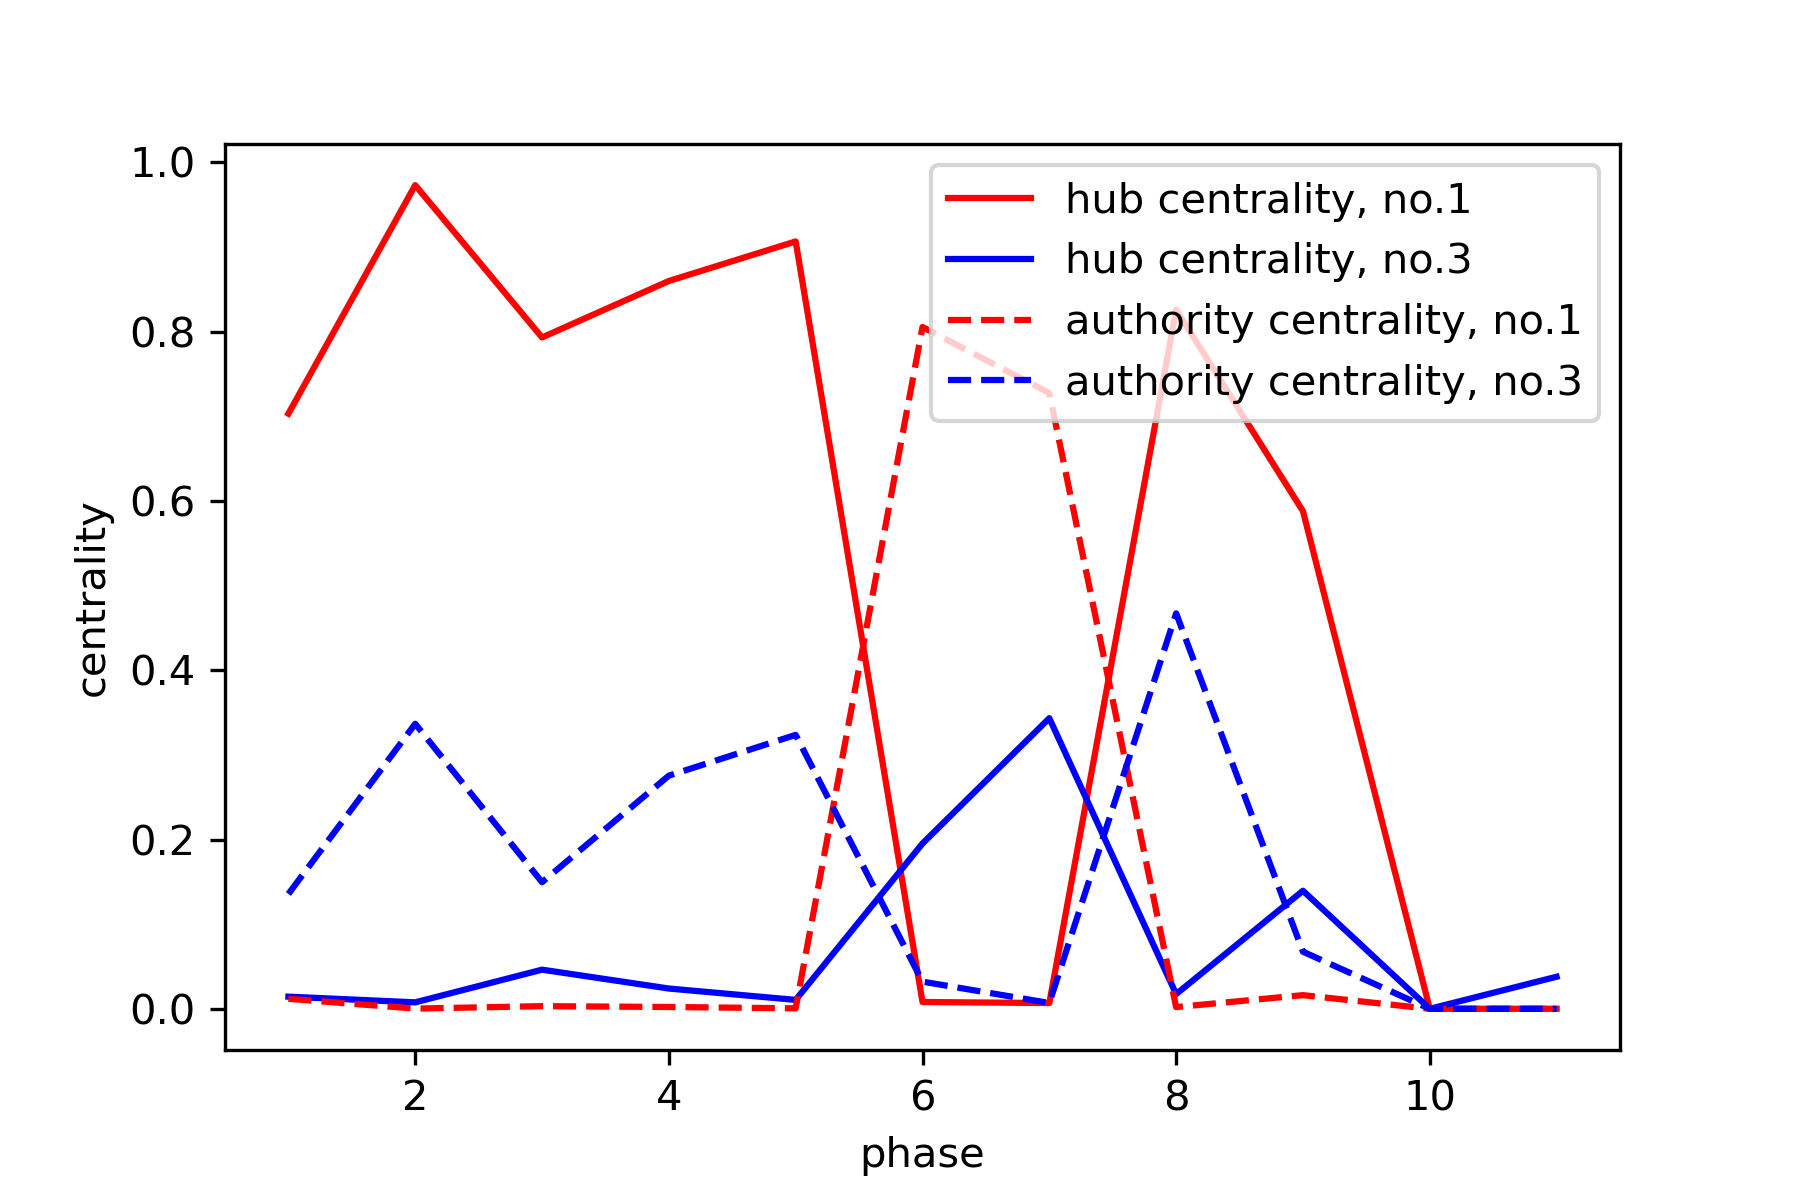
\includegraphics[width=0.7\linewidth]{problem_02/hubs_authorities}
	\caption{Hub and authority centrality for nodes no.1 and no.2}
	\label{fig:hubs_authorities}
\end{figure}

For both nodes there is the correlation that the hub centrality increases with an decreasing authority centrality, vice versa (see figure \ref{fig:hubs_authorities}). Moreover, the centralities for both nodes seem to be correlated as well. When there is an decrease in hub centrality for node no. 1 the hub centrality of node no. 3 increases. The same pattern can be found for the authority centrality. In other words, if for example the importance of outgoing messages of node no. 1 is reduced (in phases of high value seizures) the importance of outgoing massages of node no. 3 increases. Node no. 3 seem to overtake some of the importance of node no. 1 in these phases. In context of the introduction this makes perfect sense, due to the position of node no. 3 in the CAVIAR network. He is the principal lieutenant of node no. 1 and in close contact to this position. He might even work as a substitute for node no. 1 in phases of costly seizures.\\

	
	\newpage
	\textbf{Problem 3 Project}\\
facebook data set - project not finished (not enough time left)\\
\textsl{This projects tries to answer several questions like it is mentioned in the suggestions.}\\
	\textsl{a) Do all given ego-networks merge together in one larger network?}\\
	\textsl{b) Are the base-nodes (or ego-nodes) for the ego-networks the most important in the merged network? Are there more important nodes?}\\

\textbf{Solution}:\\
The data set represents 10 users with their friends on the facebook network\cite{facebook_data}. The data is stored in several files. The connections between one node and its friends is stored in the nodeId.edges files. The data in these files contains the edges (or friendships) between the nodeId's sub-nodes (or friends). By doing that, the network is split into several "ego-networks". By merging the 10 .edge files and adding the connections between ego-nodes and their friends, we receive the whole network for this project.\\

The question a) states, that all sub-graphs are connected. This can be assumed due to the small introduction, but shall be proven visually in this matter. The graph can be seen in figure \ref{fig:facebook_network_global}. Without any further explanation we see that there are no nodes which are not connected within the network.\\

\begin{figure}[h]
	\centering
	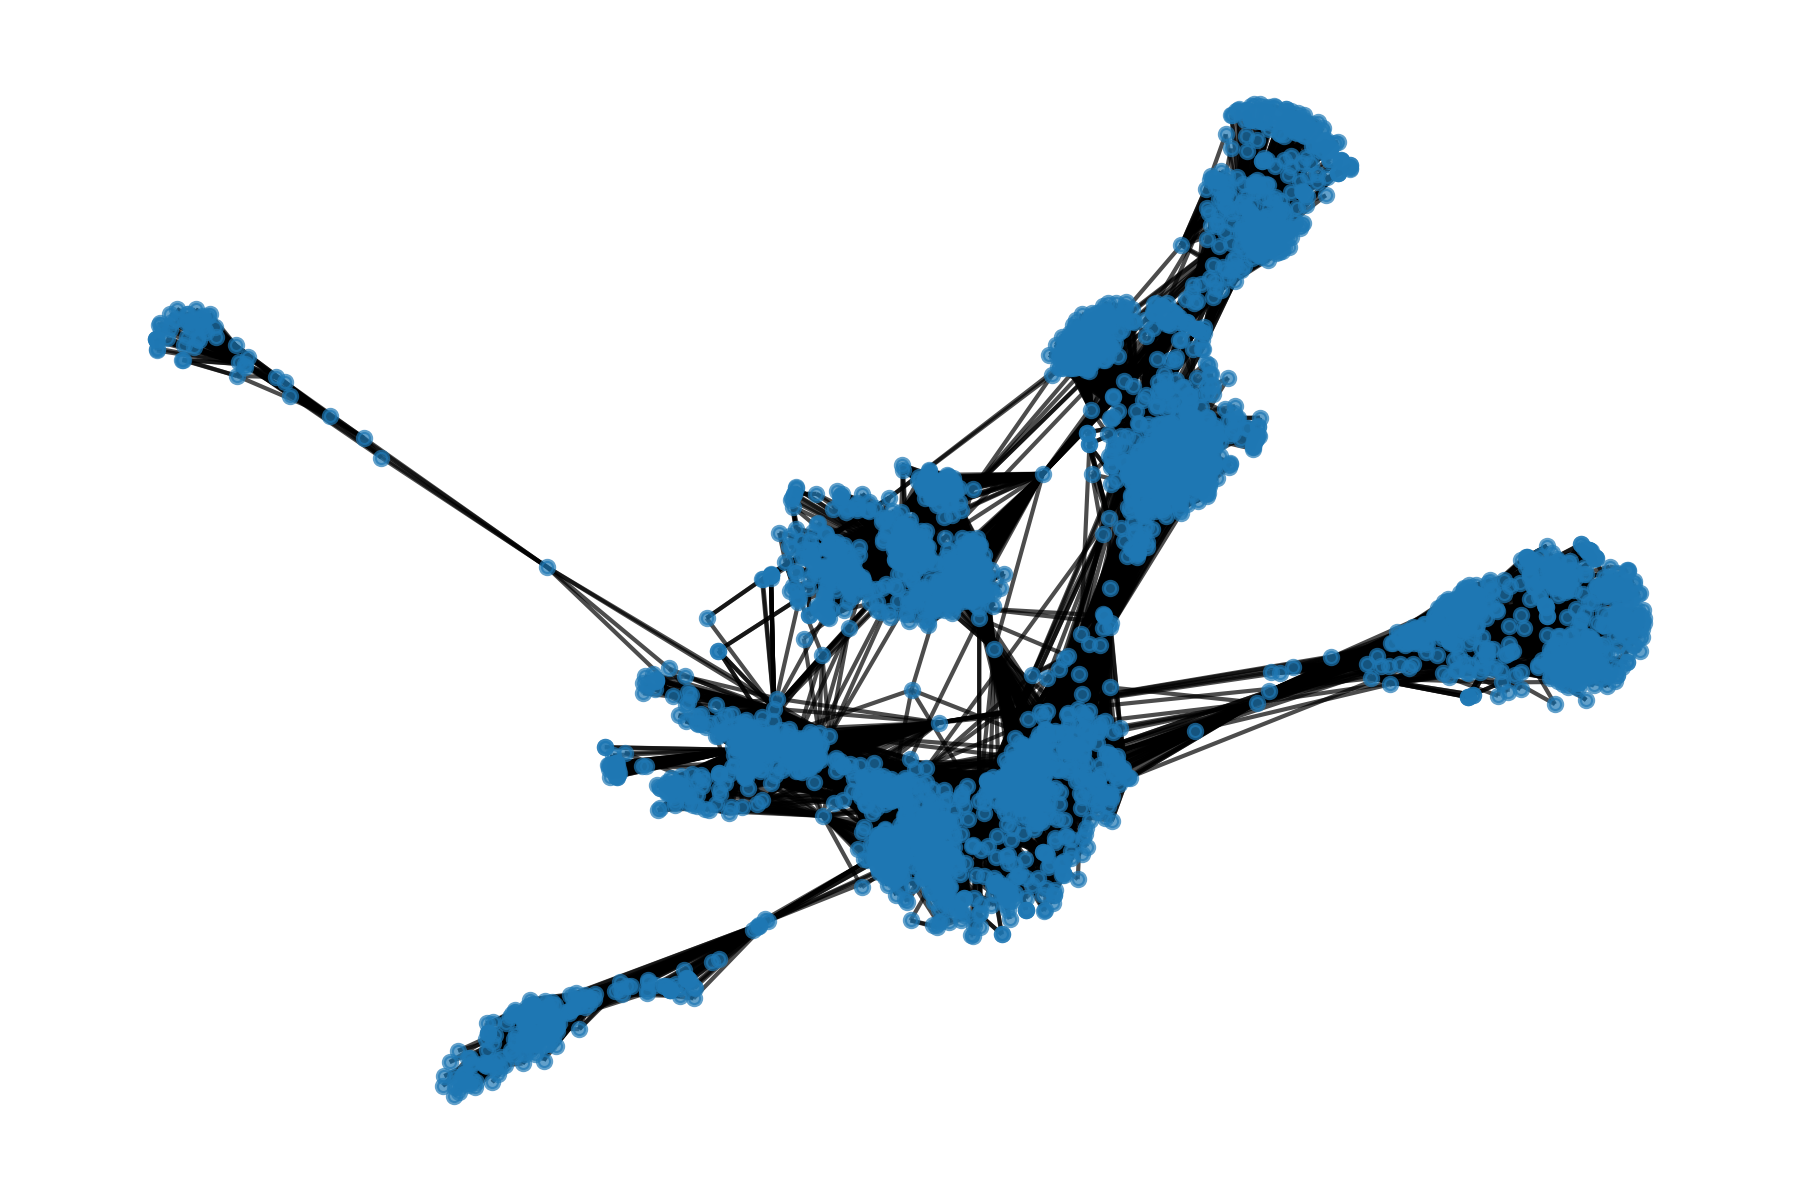
\includegraphics[width=0.7\linewidth]{problem_03/facebook_network_global}
	\caption{Connected nodes (10 representative nodes with their ego-networks)}
	\label{fig:facebook_network_global}
\end{figure}

To answer question b) we need to define on which criterion the importance of a node is defined. We have several possibilities for this definition. To answer the question I will list the ego-nodes, ordered by importance according to the ego-network node count or the degree of the ego-node\footnote{Due to the undirected network, the in-degree is equivalent to the out-degree.}. Next, I will compare this list with the degree of all nodes, the eigenvector and the betweenness centrality of the 10 nodes of highest centrality.\\

As the table \ref{tab:importance_nodes} shows, the ego-nodes are not necessarily the most important nodes according to the before mentioned centrality measures. The degree is a poor criterion to judge whether other nodes are more important than ego-nodes. Nodes in larger ego-networks generally reach higher degrees, irrelevant if the node is an ego-node or a plain sub-node within the ego-network due their numerous connections. 

\begin{table}[h]
	\centering
	\begin{tabular}{|c|c|}
		\hline 
		Degree (ego-nodes) 	& Degree (all nodes)\\ 
		$[$edge count$]$ 	& $[$edge count$]$\\ 
		\hline 
		no.107 (1034) 		& no.107 (1034)\\ 
		\hline 
		no.1684 (786) 		& no.1684 (786)\\ 
		\hline 
		no.1912 (747)		& no.1912 (747)\\ 
		\hline 
		no.3437 (534) 		& no.3437 (534)\\ 
		\hline 
		no.0 (333)    		& no.0 (333)\\ 
		\hline 
		no.348 (226)  		& no.2443 (294)\\ 
		\hline 
		no.686 (168)  		& no.2347 (291)\\ 
		\hline 
		no.414 (150)  		& no.1888 (254)\\ 
		\hline 
		no.698 (63)			& no.1800 (245)\\ 
		\hline 
		no.3980 (52)		& no.1663 (235)\\ 
		\hline 
	\end{tabular} 
	\caption{Comparison of different nodes according to importance (left to right: degree of ego-nodes and all nodes, (missing: eigenvector centrality, betweenness centrality))}
	\label{tab:importance_nodes}
\end{table}
	
	\newpage
	\renewcommand{\bibname}{References}
	
	\begin{thebibliography}{}
	
	\bibitem[1]{sparse_matrix} https://math.stackexchange.com/questions/2981167/time-complexity-for-sparse-matrix-multiplication-xxt
	\bibitem[2]{networks_an_introduction}
	Newman, M.E.J.; Networks An Introduction. 2010, Oxford University Press
	\bibitem[3]{facebook_data}
	https://snap.stanford.edu/data/ego-Facebook.html

	\end{thebibliography}


\end{document}